\chapter{Outer detector commissioning and monitoring}\label{chap:ODCommissioning}
The Outer Detector (OD) of the LUX-ZEPLIN (LZ) experiment plays a critical role in suppressing backgrounds for the direct detection of Weakly Interacting Massive Particles (WIMPs). Composed of ten acrylic vessels filled with gadolinium-loaded liquid scintillator (GdLS) and optically coupled to photomultiplier tubes (PMTs), the OD is primarily designed to identify and veto neutron backgrounds that mimic WIMP signals in the Time Projection Chamber (TPC). This chapter presents the OD PMT single photon electron calibration in \autoref{sec:ODCommissioning/PMTCalibration} and in \autoref{sec:ODComissioning/RecGain} describes the method which is used to reconstruct the gain of the OD PMTs. Finally, \autoref{sec:ODCommissioning/OCSDevelopment} details the development of the OD optical calibration system (OD OCS) and its monitoring PMT which is used to monitor the stability of the light used to calibrate the OD PMTs.

\section{OD PMT calibration}\label{sec:ODCommissioning/PMTCalibration}
As discussed in \autoref{sec:LZ/LZOD}, the primary purpose for the OD is to detect neutron interactions which have coincident signals within the TPC. Neutrons in a MeV range are produced in radioactive decays via spontaneous fission (SF) and ($\alpha$, n) reactions and by cosmic rays. However, neutron fluxes from radioactivity dominate LZ's neutron background as the experiment is located deep underground. Neutrons from atmospheric showers do not penetrate hundreds of meters of rock whilst muon-induced neutrons are tagged using coincident detection of the muon which initiated the cascade \cite{LZ_SIMS}.

SF occurs in heavy nuclei where the nucleus dissociates spontaneously into two roughly equal parts. This fission is accompanied by the emission of neutrons and gamma rays. Among naturally occurring radioisotopes, only fission of \textsuperscript{238}U contributes significantly to neutron production via SF \cite{Kudryavtsev:2020eer}.

Two radioactive decay chains are primarily responsible for the neutron background resulting from ($\alpha$, n) reactions. These chains start with the parent isotopes of \textsuperscript{238}U and \textsuperscript{232}Th and consist of 6 and 8 alpha-decays, respectively \cite{Kudryavtsev:2020eer}. An alpha particle from the decay collides with a target nucleus, causing the emission of a neutron. Calibration sources are produced which benefit from this reaction (see \autoref{sec:VetoEff/NeutronsFromCalibrationSources}) however rare event search experiments need to mitigate against ($\alpha$, n) reactions which occur in detector materials.

A neutron produced by SF or by an ($\alpha$, n) reaction will enter the xenon and then scatter out. The neutron then traverses the intervening material thermalizing and captures on either the gadolinium or the hydrogen in the GdLS, or recoils off protons. Neutron recoils produce energy depositions of $\sim$100~keV \cite{LZNIMA}. The pulses of light detected in the PMTs for such low energy interactions are $\sim$15 photons in size and require the PMTs to be calibrated to a single photon sensitivity. Understanding the response of the PMTs is key to measuring single photon sensitivity and in turn reconstructing the gain of the PMTs. A model of photomultiplier response is presented in Ref.~\cite{BELLAMY1994468} which will be described below.
\subsection{Single photoelectron response model}\label{sec:ODComissioning/SPhEResponse}
The PMT can be modelled as consisting of two independent parts:
\begin{itemize}
    \item A photo-cathode where photons are converted into electrons
    \item An amplified which amplifies the initial charge (dynode system)
\end{itemize}
The model \cite{BELLAMY1994468} assumes that the number of photons incident on the PMT and subsequently the photo-cathode is a Poisson distributed variable. Only a fraction of the photons are converted to photoelectrons, this is the quantum efficiency of the PMT and is a random binary process ($\sim~25\%$ for the OD PMTs). The photoelectrons are then guided towards the first dynode by an electric field in which $\mathcal{O}(100\%)$ photoelectrons complete this process. The convolution of the Poisson and binary process results in a Poisson distribution:
\begin{equation}\label{eqn:SPEPoiss}
    P(n;\mu)=\frac{\mu^{n}e^{-\mu}}{n!},
\end{equation}
where $\mu$ is the mean number of photoelectrons collected at first dynode, $P(n;\mu)$ is the probability that $n$ photoelectrons are observed for a mean $\mu$.
The photoelectron is then amplified by the dynode system, which for the OD PMTs is a series of 10 dynodes. The amplification of the dynode system to determined by the voltage distribution across the dynode and it is tuned on a PMT-by-PMT basis to achieve a gain of $\mathcal{O}(10^6)$. The cascade of photoelectrons produced from the amplification is collected at the anode of the PMT and a voltage is measured as a pulse. The area of the pulse corresponds to number of electrons incident on the anode and is expressed as a Gaussian distribution:
\begin{equation}\label{eqn:SPEGauss}
    G_n(x)=\frac{1}{\sigma_1\sqrt{2n\pi}}exp\biggl(-\frac{(x-nQ_1)^2}{2n\sigma_1^2}\biggl),
\end{equation}
where $x$ is the variable charge, $Q_1$ is the mean value of the charge outputted from the amplification at the dynode, $\sigma_1$ is the standard deviation of the charge amplification.
The response of an ideal PMT, $S_{ideal}$, can be described simply by convoluting \autoref{eqn:SPEPoiss} and \autoref{eqn:SPEGauss} together:
\begin{equation}
    \begin{split}
    S_{ideal}(x) & = P(n;\mu)\otimes G_n(x) \\
    & = \sum^\infty_{n=0}\frac{\mu^{n}e^{-\mu}}{n!}\frac{1}{\sigma_1\sqrt{2n\pi}}exp\biggl(-\frac{(x-nQ_1)^2}{2n\sigma_1^2}\biggl),
    \end{split}
    \label{eqn:PoisPlusGauss}
\end{equation}
the model is summed from 0 photons to an arbitrary upper limit \cite{BELLAMY1994468}.
\subsection{Single photoelectron calibration}\label{sec:ODComissioning/SPhECalib}
To calibrate the OD Single photoelectron (SPhE) response, 435~nm light is injected into the OD using the ODOCS. The optimal intensity of light to induce a SPhE response is chosen during the commissioning of the OD following the PMT installation in 2021. Details of the optimisation can be found in Ref.~\cite{edfraser:thesis}.

Due to the geometry of the OD, the central row fibres are chosen as the injection points, position 2 in \autoref{fig:LZ/OCSPositions} (central row). Light injected from the central row fibres pass through the side acrylic tanks (SATs) and reflects back of the Tyvek layer which covers the OCV.
Light injected from position 1 has the ability to pass direct through the top acrylic tanks (TATs). Light injected from position 3 is reflected within the bottom acrylic tanks (BATs) due to Tyvek layers which was placed between the three acrylic tanks to cover foam which was needed to displace water. This later design decision was to increase light collection. Irregular gaps between BATs are present due to differences in moulding during construction of the BATs.

The OCS in configured so that 1000~photons are emitted from the end of the fibre. Due to attenuation of light in the fibre, 2000~photons must be emitted by the LEDs to account for a factor of two attenuation. For each injection of light, one of the 10 central row fibre emits 200,000~pulses at a 700~Hz injection rate. The rate of pulses injected was determined to not overload the LZ DAQ.

For ease of repeated measurement, an analysis module for the OD SPhE was developed to be used in conjunction with the LZ Physics Readiness Monitor (PREM) \cite{LZTDR}. The analysis module contains a selection to identify the OCS pulse and differentiate it from the background light seen in the OD. It be seen in \autoref{fig:ODCommissioning/ODSPhE_TimingSelection} that the OCS pulses are distributed around a peak at 560~ns after the trigger, which corresponds to 0~ns in \autoref{fig:ODCommissioning/ODSPhE_TimingSelection}. A selection of pulses with occurred between 500~ns and 700~ns after the DAQ was triggered by the OCS was chosen as an appropriate set of bounds for the timing selection to identify the OCS pulse. A PMT coincidence requirement was also imposed to improve the purity of the selection as pulses with a coincidence greater than 1 PMT would likely not include any afterpulses which could mimic an OCS pulse.

\begin{figure}[ht!]
    \centering
    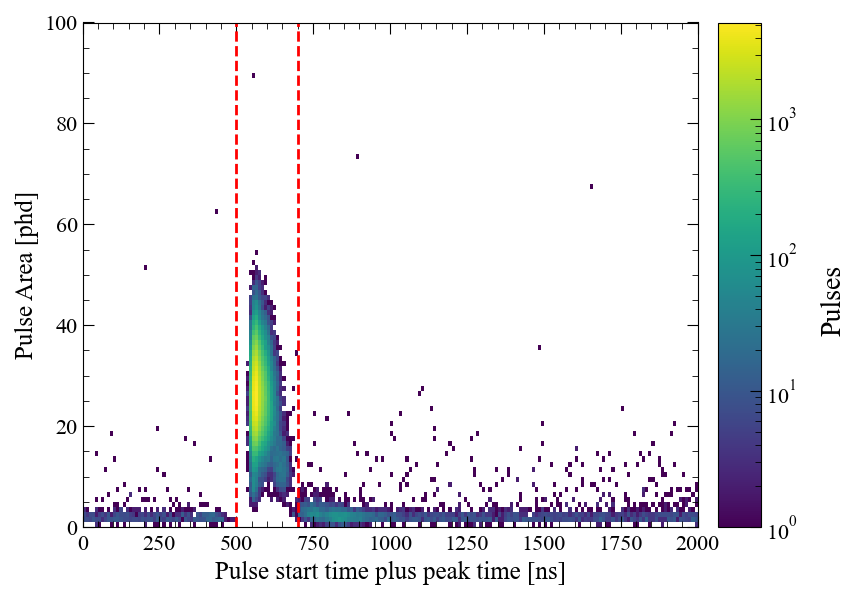
\includegraphics[width=0.7\linewidth]{figures/ODCommissioning/TimingVsPulseArea_2us.png}
    \caption{The response of the OD PMTs to 200,000 injections of 2000 photons during a monthly SPhE measurement. The pulse area is plotted against the start time of the pulse relative to the trigger plus the peak time relative to the start of the pulse. The OCS pulses are distributed around a peak of 560~ns. The two vertical dashed red lines indicate the inclusive timing selection criteria.}
    \label{fig:ODCommissioning/ODSPhE_TimingSelection}
\end{figure}


To measure the OD PMT's SPhE response \autoref{eqn:PoisPlusGauss} was used to fit the channel pulse area distributions. A two-stage fitting procedure was employed to account for the monthly variation in SPhE size across all 120 OD PMTs. The first stage of the procedure, only the single SPhE peak is fitted. Initially during commissioning, the starting value for $-\mu$ was determined by estimating the proportion of events in which no photon would be measured by the PMT. The mean ($\mu$) and standard deviation ($\sigma$) of the histogram was used as starting values for components of the initial fit. The normalisation was taken to be the area beneath the curve between $\mu/4$ and $6\cdot\mu$. The range in which to apply the fit was determined using the peak and defined from $\mu\pm(\sigma/\mu)$. In the second stage of the fitting procedure, the parameters from the initial fit were used as starting parameters to a fit of the multiple SPhE distribution. The range in which to apply the second stage fit was from $\mu-\sigma$ to $\mu+3\cdot\sigma$. For each run only one fibre is used to inject light resulting in a small percentage of bad fits across the 120 PMTs depending on the particular fibre being used relative to the PMT of interest. To filter out such bad fits, only fits with $\chi^2/\text{ndf}<3$ were recorded for further analysis.

An example histogram and fit can be seen in \autoref{fig:ODCommissioning/ODSPhEDists}. We see that the OD PMTs exhibit the expected response to SPhE as discussed in \autoref{sec:ODComissioning/SPhEResponse}

\begin{figure}
     \centering
     \begin{subfigure}[b]{0.47\textwidth}
         \centering
         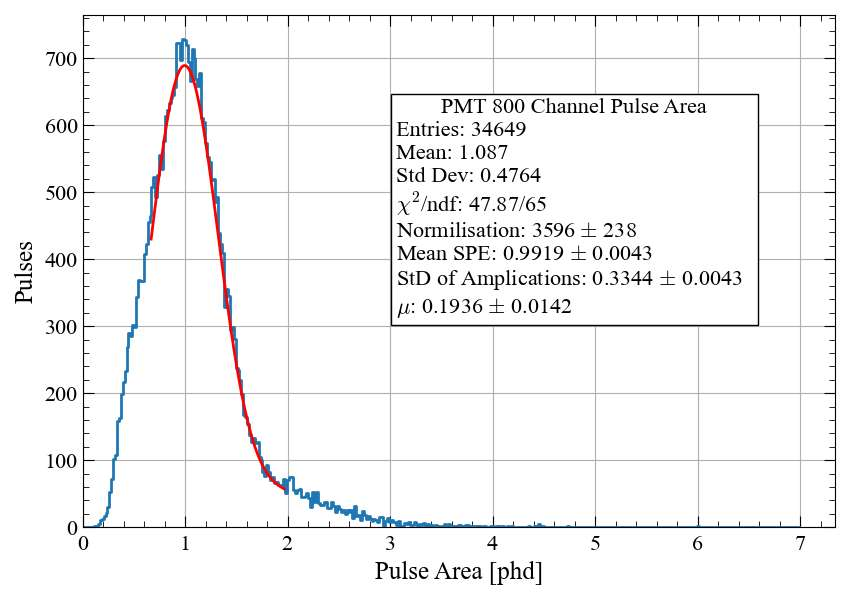
\includegraphics[width=\textwidth]{figures/ODCommissioning/PMT800_PulseArea_Distribution.png}
         \caption{}
         \label{fig:ODCommissioning/ODSPhE_phd}
     \end{subfigure}
%     \hfill
     \begin{subfigure}[b]{0.47\textwidth}
         \centering
         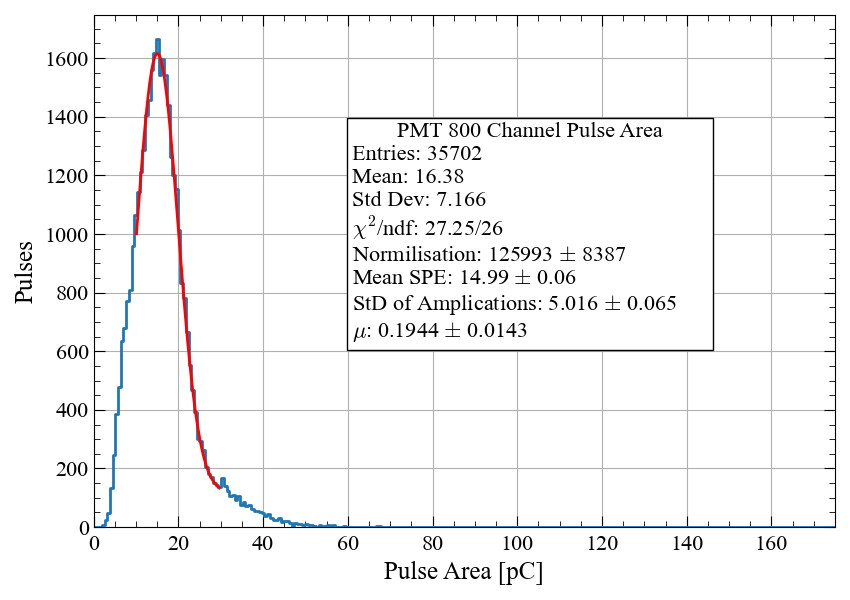
\includegraphics[width=\textwidth]{figures/ODCommissioning/PMT800_PulseArea_Distribution_pC.png}
         \caption{}
         \label{fig:ODCommissioning/ODSPhE_pC}
     \end{subfigure}
        \caption{Pulse area distributions of PMT 800 from 200,000 OCS injections of 2000 photons during OD SPhE measurement. \textbf{Left:} Reconstructed pulse area measured in photons detected. \textbf{Right:} Pulse area taken from the area measured in the raw waveform in mVns, and converted to pCns by dividing by the $50~\Omega$ termination at the amplifier. The fit applied in red is \autoref{eqn:PoisPlusGauss} and the constants can be seen in the respective statistics boxes on each plot.}
        \label{fig:ODCommissioning/ODSPhEDists}
\end{figure}
An example PMT calibration is outlined below for PMT 800. The mean Gaussian response is (0.9919 $\pm$ 0.0043) phd and (14.99 $\pm$ 0.06) pCns. The SPhE calibration constant used to process the raw data is reconstructed by dividing the SPhE response measured in mVns by the SPhE response measured in phd, which in this case for PMT 800 is 753.9~mVns. These three values together are stored in the PREM database. In a secondary analysis stage, the measured SPhE area and calibration constant are combined to get the correct SPhE constant in mVns which in this example is 748.5~mVns. The average is taken of the corrected SPhE constant for all 10 measurements corresponding to the 10 central row OCS fibre injections. The new SPhE constant is then transferred to the LZ Conditions Database along with the data and time period for which this constant is valid for. As LZ then continues to collect data, the raw pulse area measured in mVns is converted to phd by dividing the raw area by the constant. Examples of the variation in measured SPhE in both phd and mVns across all 120 PMTs is shown in \autoref{fig:ODCommissioning/SPhEValues_phd} and \autoref{fig:ODCommissioning/SPhEValues_pC}.
\begin{figure}[ht!]
    \centering
    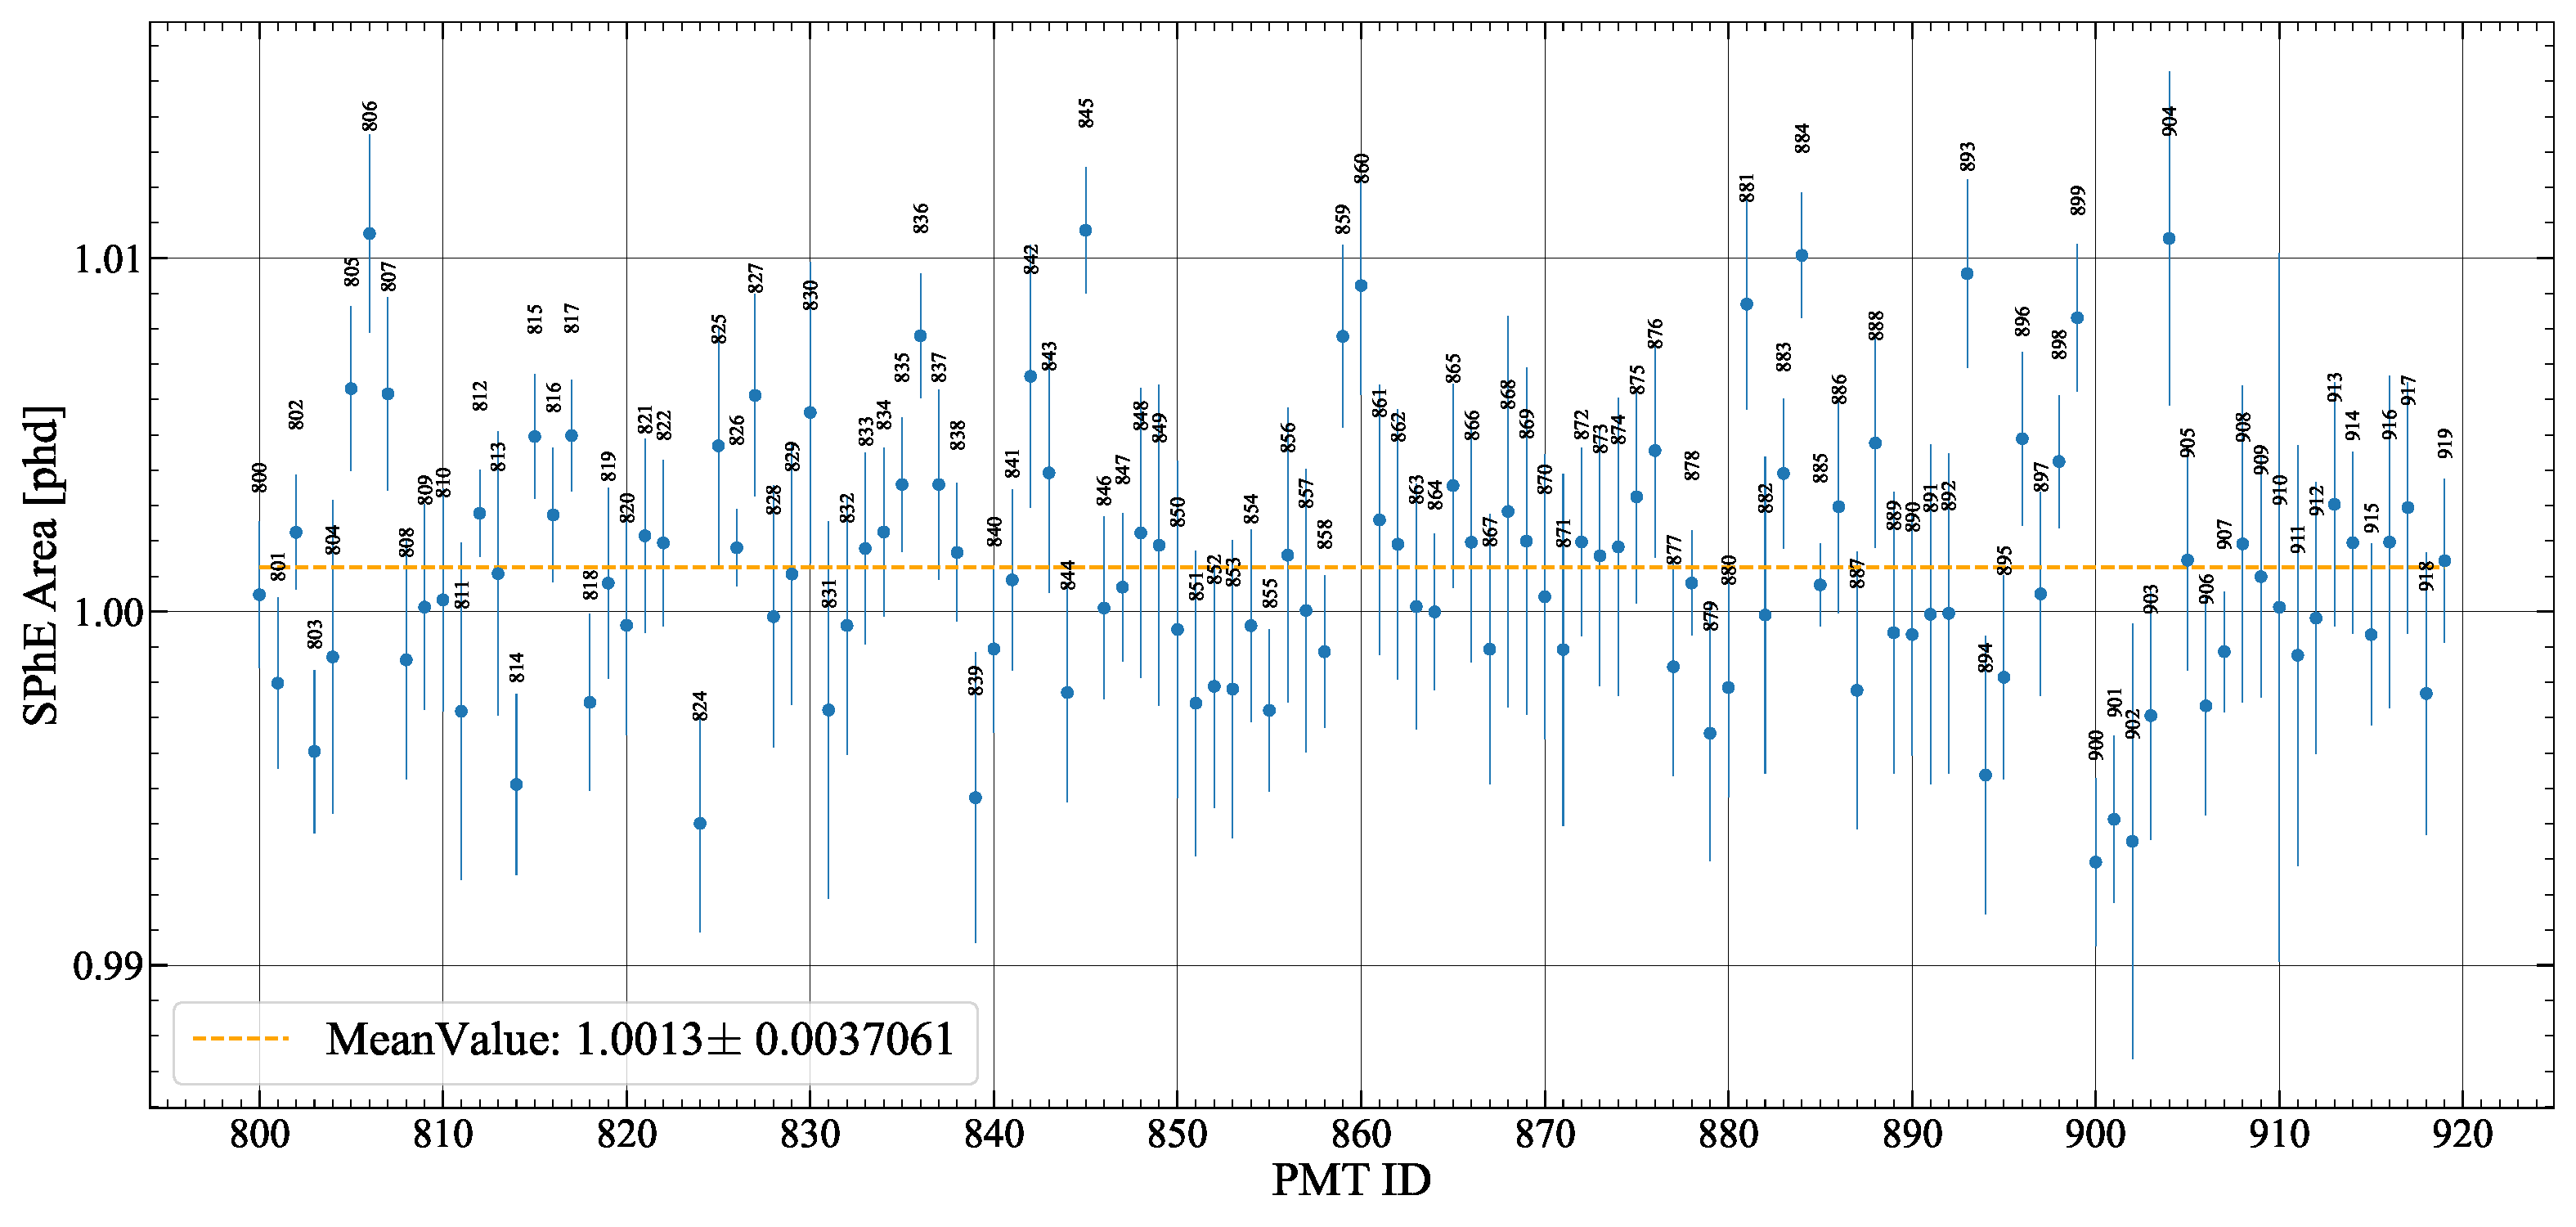
\includegraphics[width=\textwidth]{figures/ODCommissioning/SPHE_phd_2024-7-10.pdf}
    \caption{A scatter plot of the OD SPhE Area size measured in phd versus PMT ID for each OD PMT from a measurement taken on July 10th 2024.}
    \label{fig:ODCommissioning/SPhEValues_phd}
\end{figure}
\begin{figure}[ht!]
    \centering
    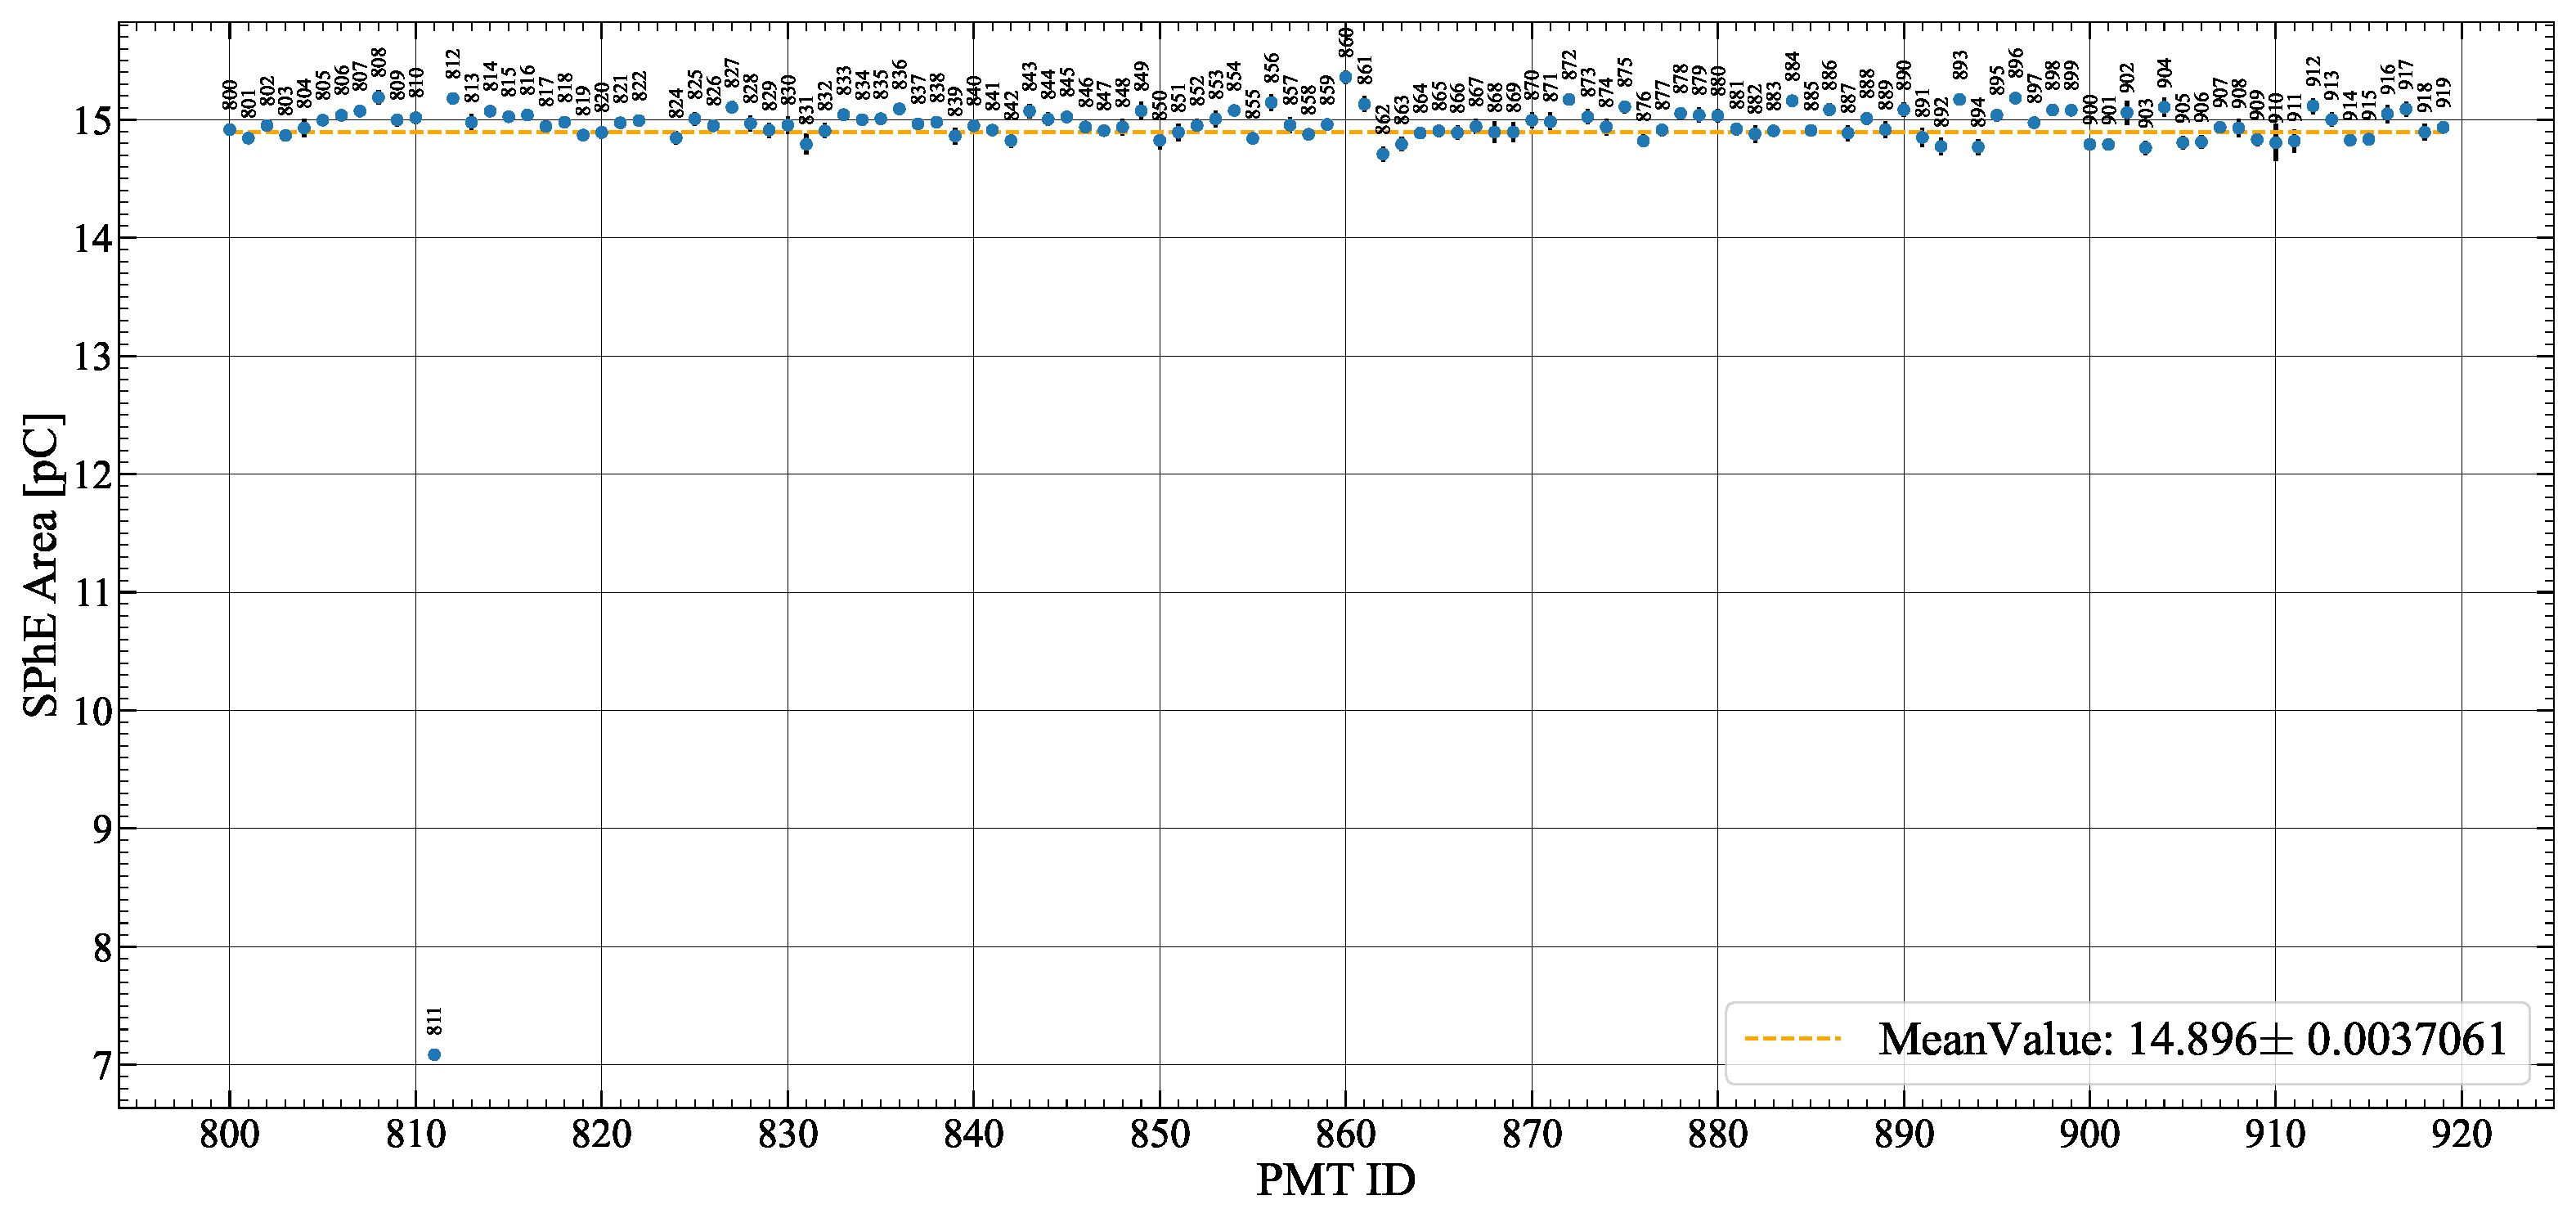
\includegraphics[width=\textwidth]{figures/ODCommissioning/SPHE_pC_2024-7-10.pdf}
    \caption{A scatter plot of the OD SPhE Area size measured in mVns versus PMT ID for each OD PMT from a measurement taken on July 10th 2024. 119 PMTs have an average SPhE area of $14.896\pm0.004$~pC, PMT 811 operating at $1\times10^6$ gain has SPhE area of $7.09\pm0.03$~pC.}
    \label{fig:ODCommissioning/SPhEValues_pC}
\end{figure}
\section{Reconstructed gain}\label{sec:ODComissioning/RecGain}
Understanding how the signal from a PMT relates to the amount of light incident on the face of the PMT is key to measuring the energy deposited by particles traversing the detector. The amplification of the photoelectrons produced through the dynode series is known as the PMT's `gain'. The SPhE Calibration Constant can be converted to understand the gain of the PMT by dividing by the following terms, $e\times44\times50\times10^{12}$, where e is the charge of an electron, $44~\text{V}_{\text{d}}$ is the total voltage division factor across all 10 dynodes in the PMT \cite{HamamatsuR5912}, 50~$\Omega$ is the termination impedance to eliminate signal reflections in the cable \cite{LZ:2024bvw}, $10^{12}$ accounts for the change with the unit prefixes on voltage and time. Using the example case from the previous section, PMT 800 had an average measured SPhE area of 748.5~mVns based on 10 OCS measurements on February $12^{\text{th}}$ 2025 which results in a reconstructed gain of $2.12\times10^6$.

During the commissioning of the Outer Detector PMT system, a target gain of $1\times10^{7}$ initially established based on the operating gain recommended by Hamamatsu Photonics \cite{LZTDR,HamamatsuR5912}. During the OD PMT QA the gain was reduced to $2\times10^{6}$ due to high rates of sub-SPhE noise. Dark rates measurements made during the QA stage exhibited significantly higher rates than the expected 1~kHz dark rate measured in off-site testing. This issue was problematic as spikes up 20~kHz were observed in some cases resulting in the LZ DAQ to crash. Final voltages corresponding to $2.1\times10^{6}$ were determined in October 2021 so that all PMTs achieved the target gain of $2\times10^6$ with $<10\%$ difference across 119 PMTs. One exception was PMT 811, whose voltage was further reduced in January 2022 resulting in a gain of $1\times10^6$ to reduce the rate of sub-SPhE pulses.
An example scatter plot of gain versus PMT ID is shown in \autoref{fig:ODCommissioning/ODPMTGain_2024-7-10}.

\begin{figure}[ht!]
    \centering
    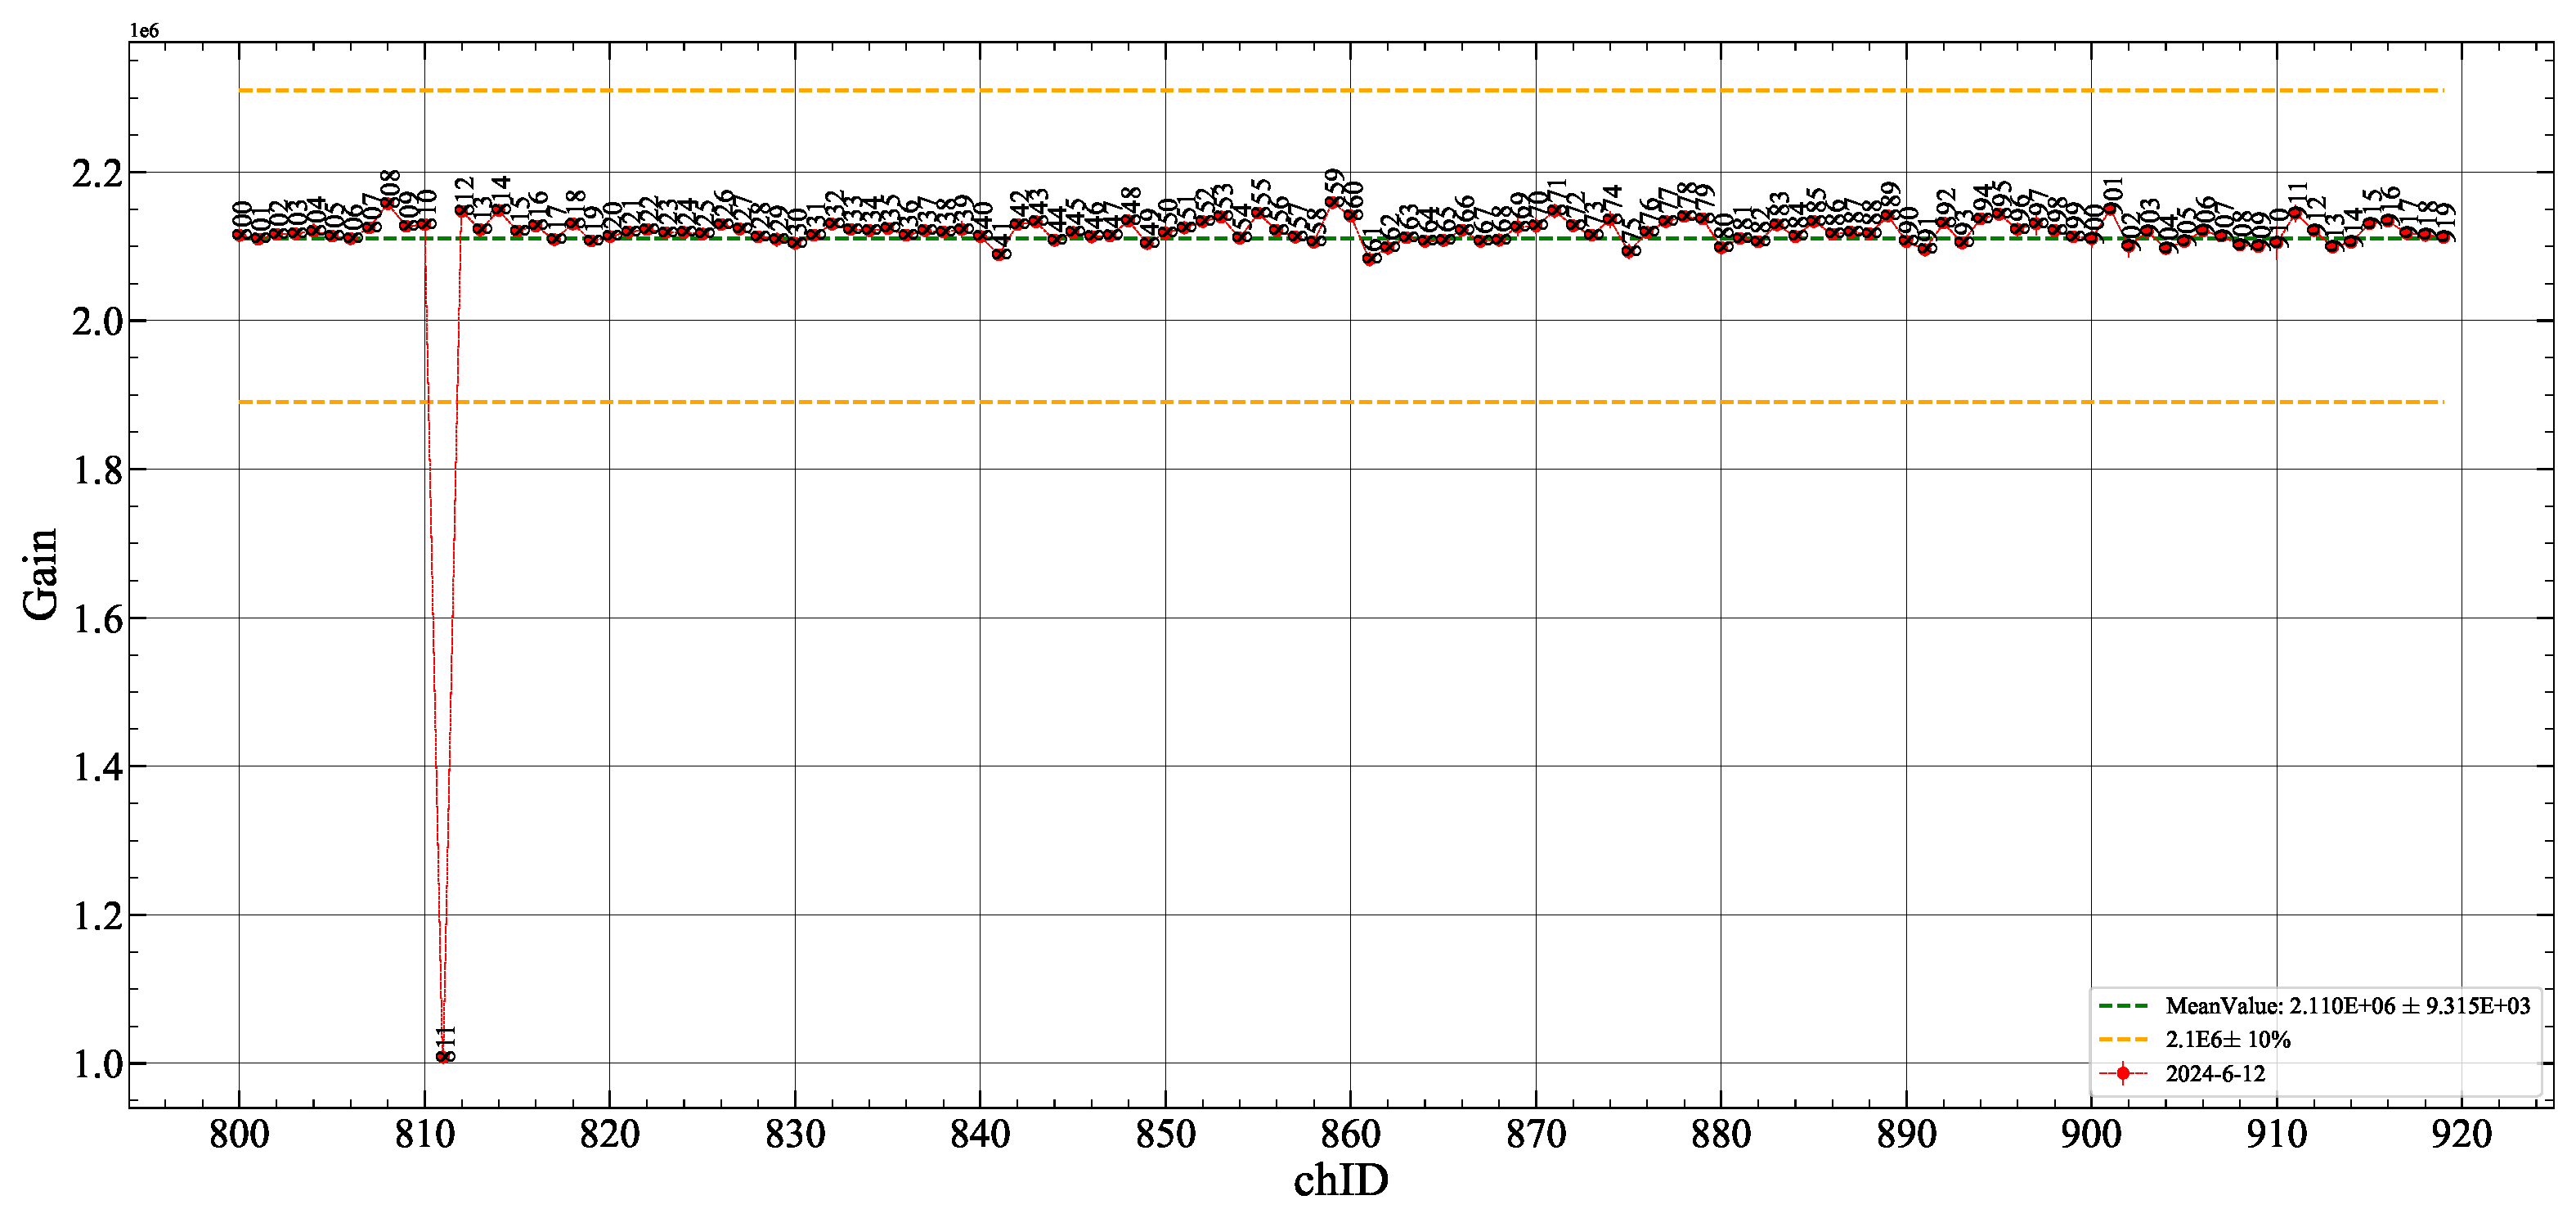
\includegraphics[width=\textwidth]{figures/ODCommissioning/2024-6-12_ODPMT_Gain.pdf}
    \caption{OD PMT Gain versus PMT ID for each OD PMT from a measurement taken on July 10th 2024. The average gain of the 120 PMTs is indicated by the dashed green line. The dashed orange lines demonstrate the $10\%$ tolerance of gain drift from $2\times10^6$ gain. PMT 811 operated at $1\times10^6$ gain is seen clearly as the outlier from the 119 PMTs operating at $\sim2\times10^6$ gain.}
    \label{fig:ODCommissioning/ODPMTGain_2024-7-10}
\end{figure}

\subsection{Monitoring PMT Response Over Time}
Whilst operating the PMTs it is important to monitoring their response as the SPhE Area size and gain can drift over time \cite{DayaBay:2016ggj,Super-Kamiokande:2023jbt}. Using the data collected during the monthly OD SPhE measurements, the distribution of gain and SPhE size was tracked throughout the science runs with gain versus PMT ID plots. The relative gain change over time during the WS2024 science run is shown in \autoref{fig:ODCommissioning/RelativeGain_WS2024}.
To monitor the observed $<1\%$ change in gain month-by-month, the relative change with respect to the start of each science run was measured. During the WS2022 science run, a mean relative change of PMT gain was measured to $(0.81\pm0.47)\%$. At the time of writing, a mean relative change of PMT gain of $(1.37\pm0.25)\%$ was measured for the WS2024 science run. Whilst the average gain change across all PMTs is relatively small, it is shown in \autoref{fig:ODCommissioning/RelativeGain_WS2024} that individual PMTs drift at different rates. Due to the short run length of WS2022 it was not necessary to adjust the PMTs voltages to gain match across the PMT array during the science run, however there was a gain matching campaign in May 2022 following the science run. Prior to the start of the WS2024 science run, the OD PMTs were gain matched again to $2.1\times10^{6}$. After 15 months of operation it was necessary to perform another gain match of the OD PMTs as PMT 859 had a relative change in gain $>10\%$ with other PMTs also approaching the $10\%$ limit set by LZ.

\iffalse
\begin{figure}[ht!]
    \centering
    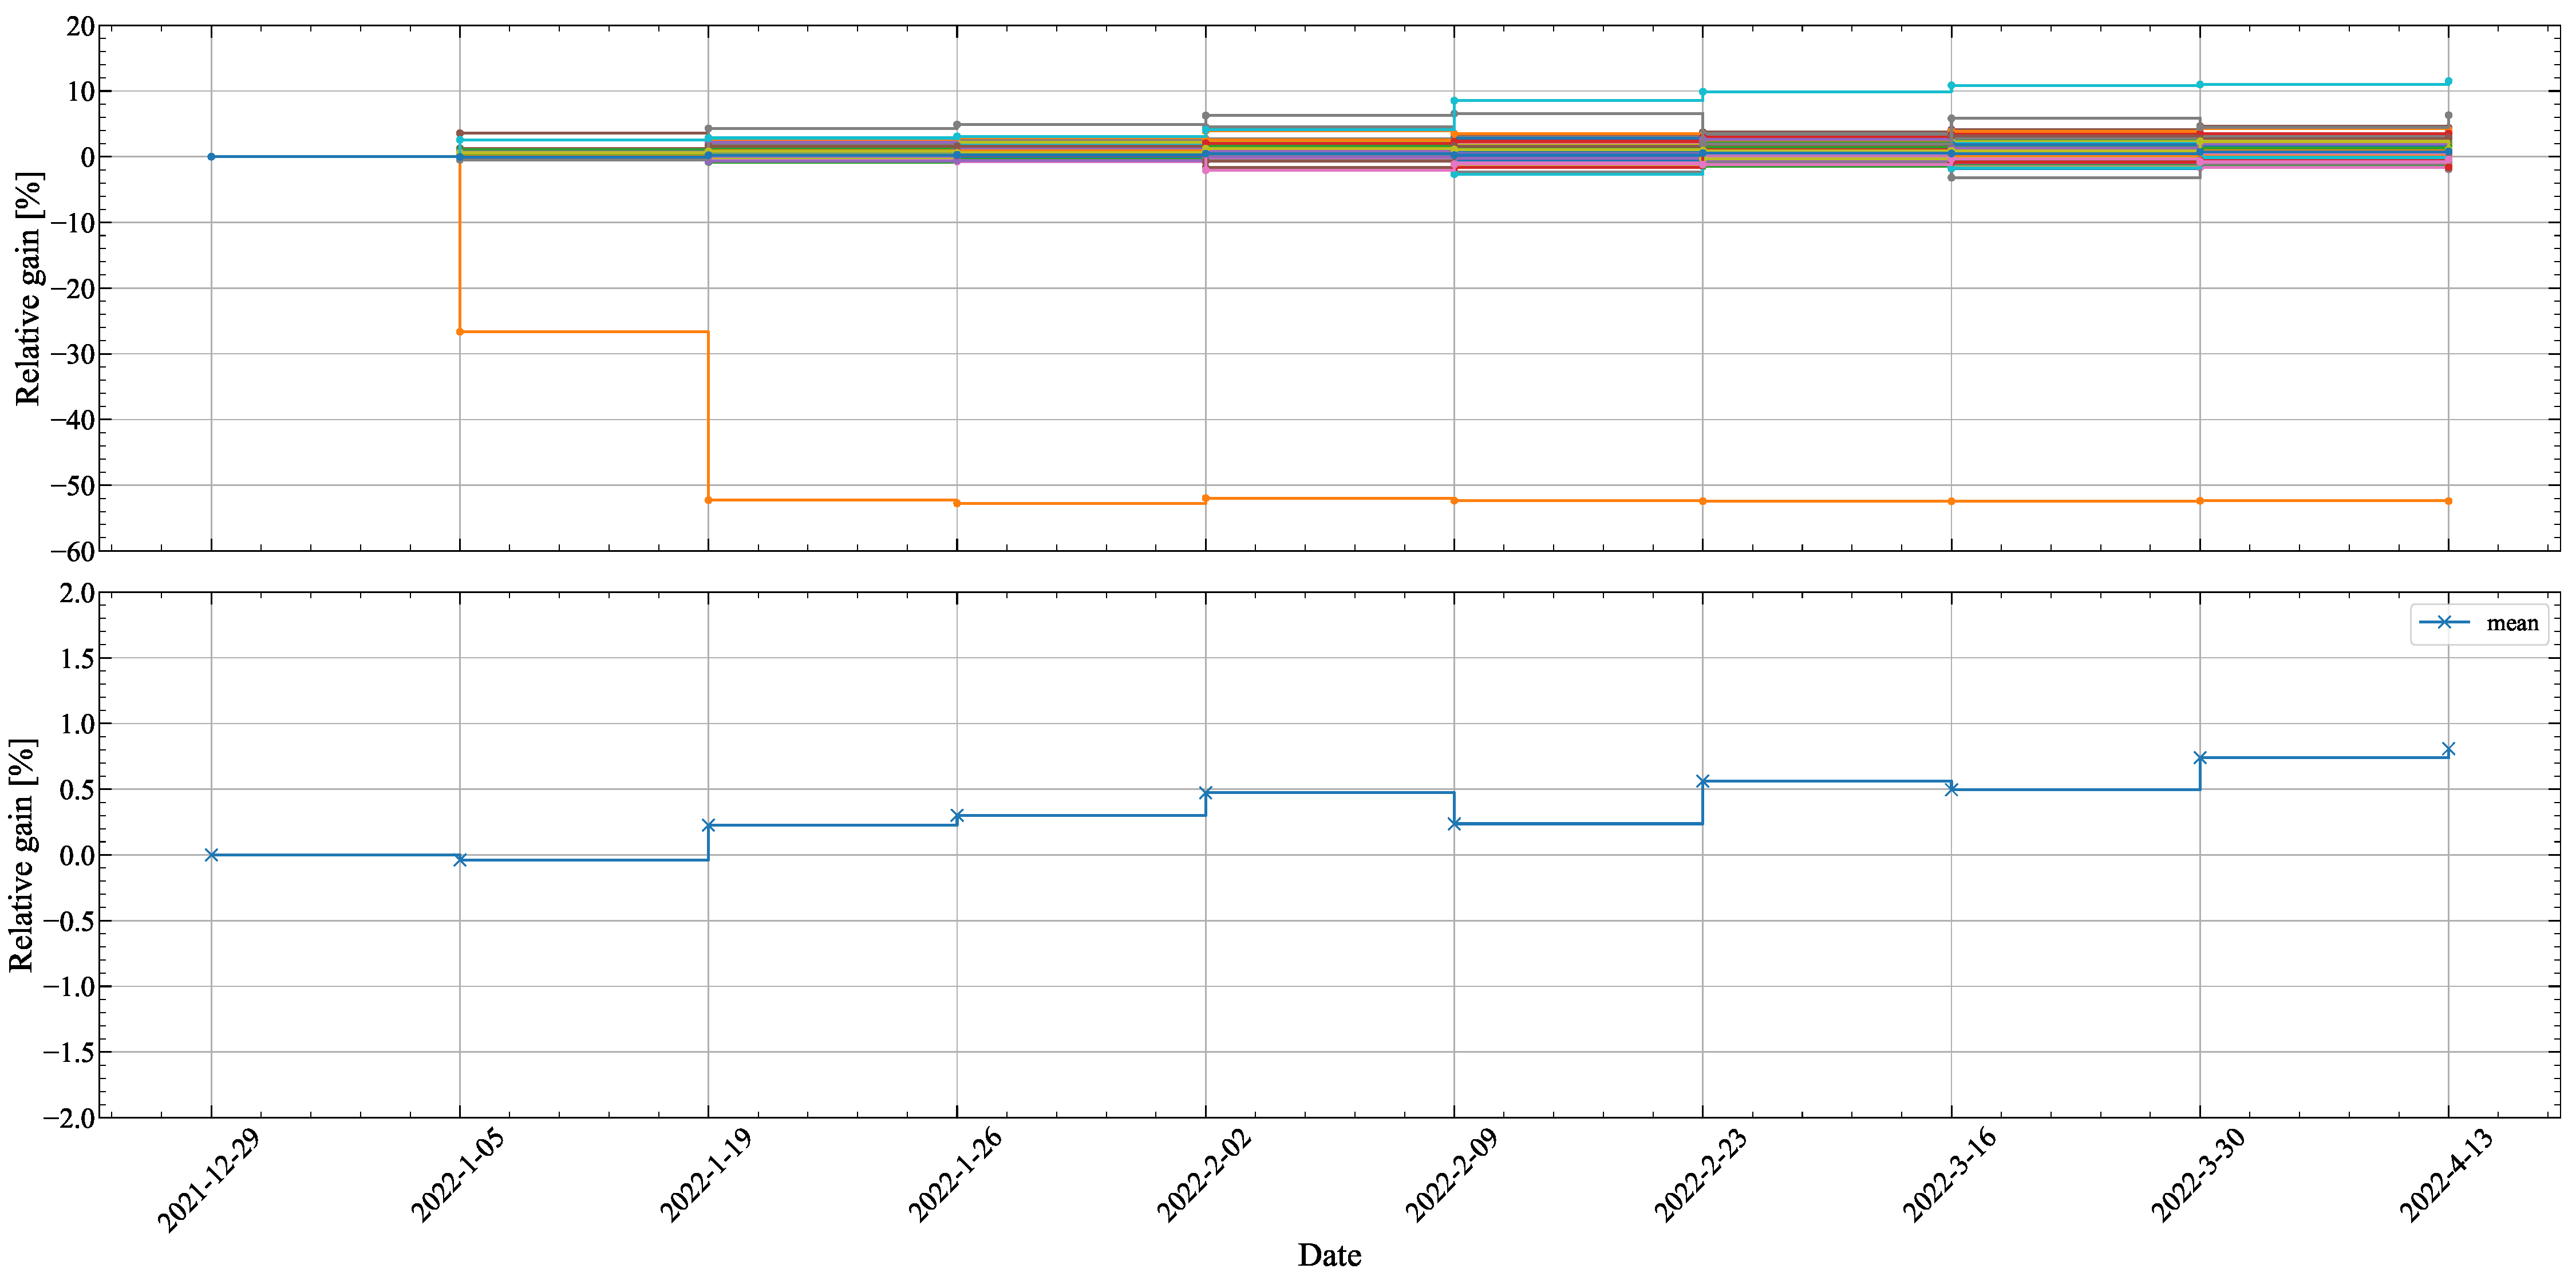
\includegraphics[width=\textwidth]{figures/ODCommissioning/RelativegainOverTime_AllPMTs_Both_Full_WS2022.pdf}
    \caption{\textbf{Top:} A scatter plot of the relative change in OD PMT Gain over WS2022 science run. The reduced gain of PMT 811 can be seen in orange. \textbf{Bottom:} A scatter plot of the average relative change in OD PMT Gain across all OD PMTs over WS2022 science run.}
    \label{fig:ODCommissioning/RelativeGain_WS2022}
\end{figure}
\fi
\begin{figure}[ht!]
    \centering
    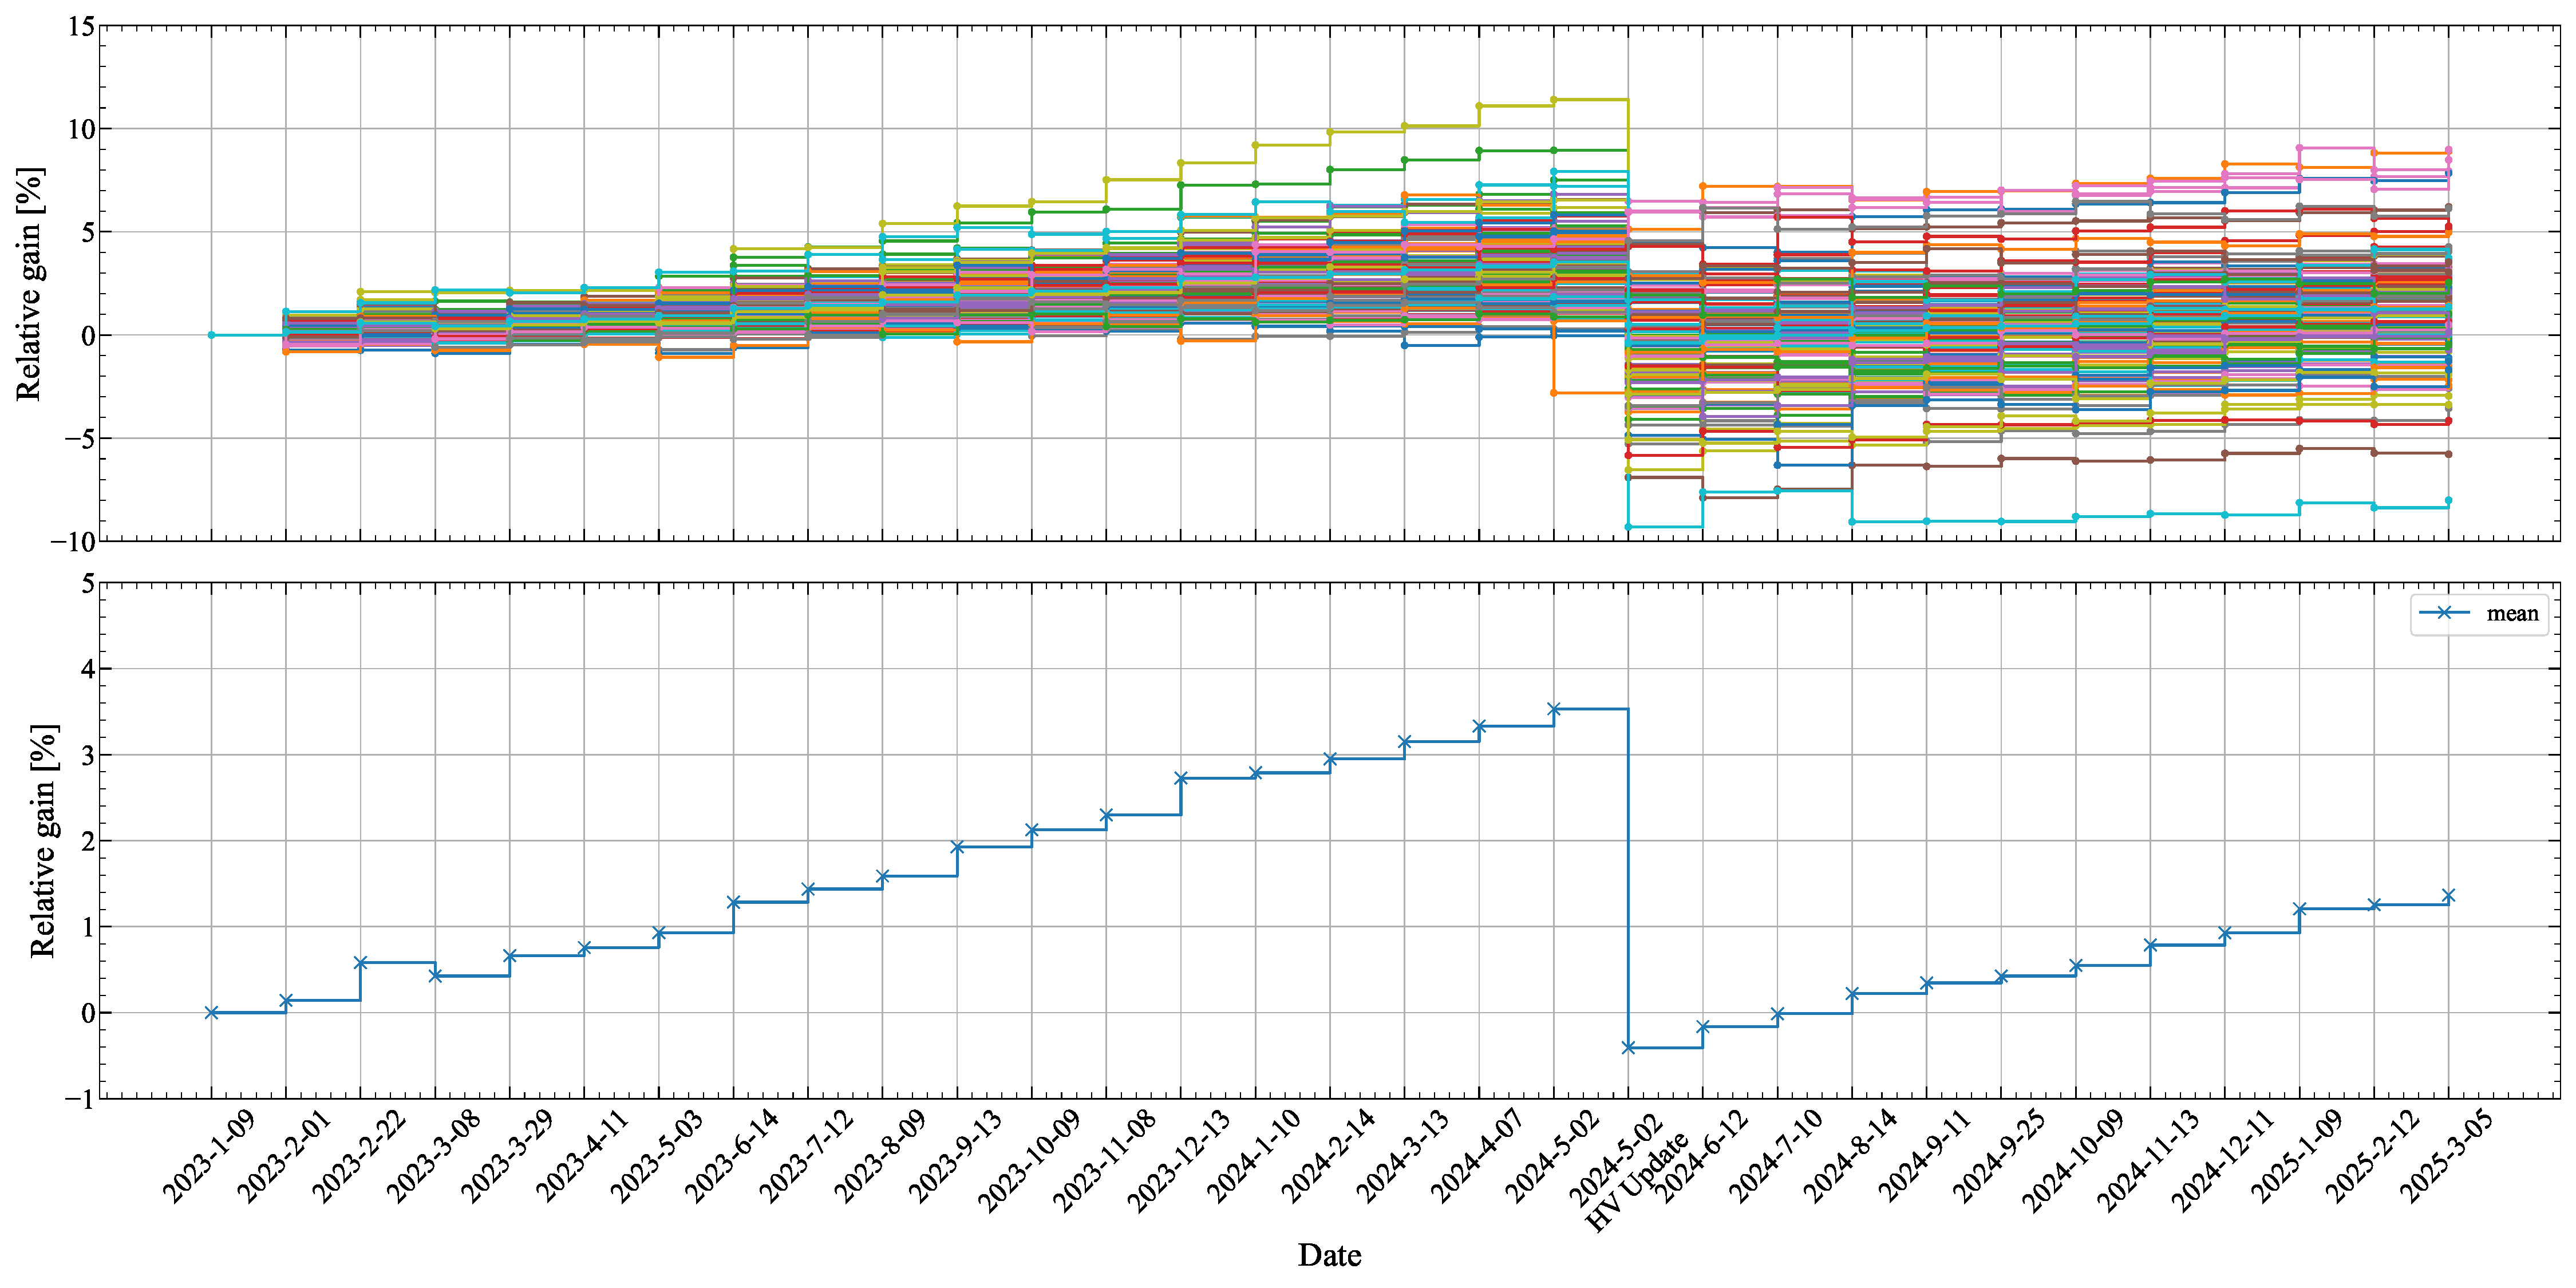
\includegraphics[width=\textwidth]{figures/ODCommissioning/RelativegainOverTime_AllPMTs_Both_Full_WS2024.pdf}
    \caption{\textbf{Top:} A scatter plot of the relative change in OD PMT Gain since the start of the WS2024 science run. \textbf{Bottom:} A scatter plot of the average relative change in OD PMT Gain across all OD PMTs since the start of the WS2024 science run.}
    \label{fig:ODCommissioning/RelativeGain_WS2024}
\end{figure}
\iffalse
\begin{figure}[ht!]
    \centering
    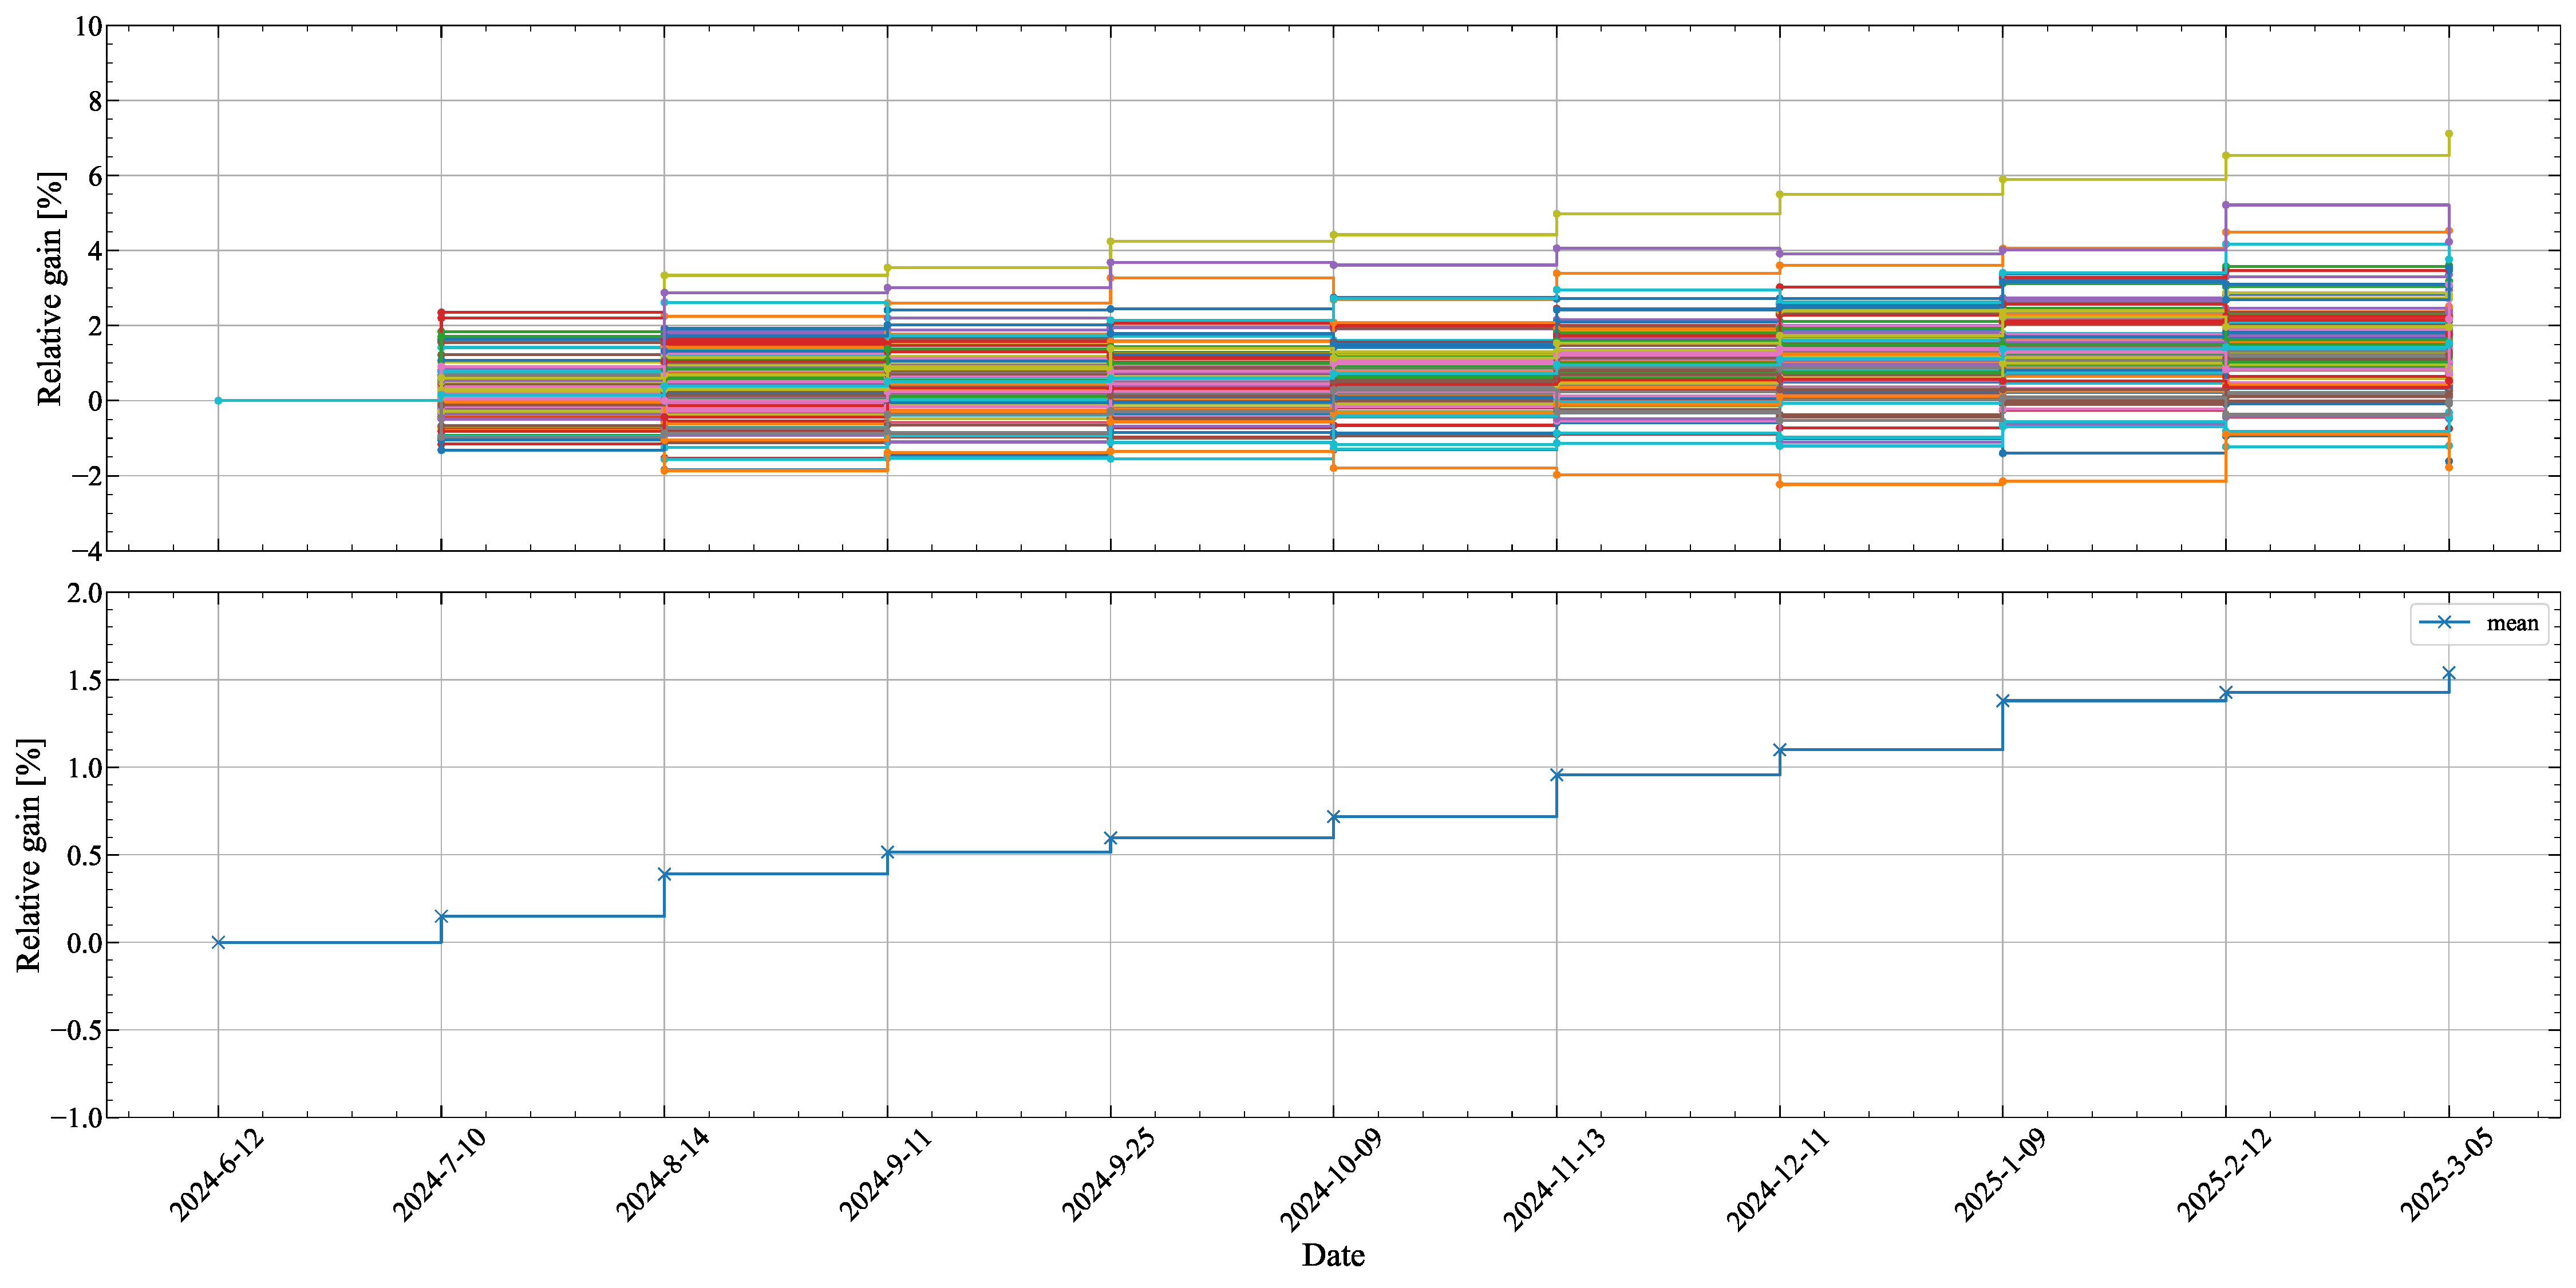
\includegraphics[width=\textwidth]{figures/ODCommissioning/RelativegainOverTime_AllPMTs_Both_Full_WS2024May2024Onwards.pdf}
    \caption{\textbf{Top:} A scatter plot of the relative change in OD PMT Gain since the gain matching campaign in May 2024. \textbf{Bottom:} A scatter plot of the average relative change in OD PMT Gain across all OD PMTs since the gain matching campaign in May 2024.}
    \label{fig:ODCommissioning/RelativeGain_WS2024May2024Onwards}
\end{figure}
\fi

\subsection{Gain Curves}
As previously discussed in \autoref{sec:ODComissioning/RecGain}, the gain of a PMT is the degree amplification of photoelectrons produced in through the dynode series. Mathematically, it can be calculated by the following equation:
\begin{equation}
    \label{eqn:GainCurve}
    \frac{G_2}{G_1}=\biggl(\frac{V_2}{V_1}\biggl)^\gamma,
\end{equation}
where $G_1$ and $G_2$ are the gains at supply voltages $V_1$ and $V_2$, $\gamma$ is a coefficient set by the dynode material and geometry (measured as 7.27 for the LZ OD PMTs). During off-site commissioning of the OD PMT array, the gain curves were determined such that the correct voltage could be chosen to achieve a desired gain of $1\times10^7$. Following the installation of the PMTs and subsequent filling of the water tank with the various detector mediums, it was seen necessary to perform a secondary measurement of the gain curves once the PMTs had been operational for six months.
Using the initial voltage ($V_{rec}$ which corresponds to $2\times10^6$ gain, five additional voltages surrounding $V_{rec}$ were chosen in 50~V spacing. For each voltage, a full SPhE measurement is made to determine the gain in each PMT. Using \autoref{eqn:GainCurve}, a new $\gamma$-factor is measured and is used for any future gain or voltage adjustment. The gain curves for PMT 800 measured prior to the start of the WS2024 campaign is shown in \autoref{fig:ODCommissioning/PMT800_gainCurve}. All gamma factors measured prior to the start of the WS2024 campaign are shown in \autoref{fig:ODCommissioning/gammaFactors}.
\iffalse
\begin{figure}[ht!]
     \centering
     \begin{subfigure}[b]{0.47\textwidth}
         \centering
         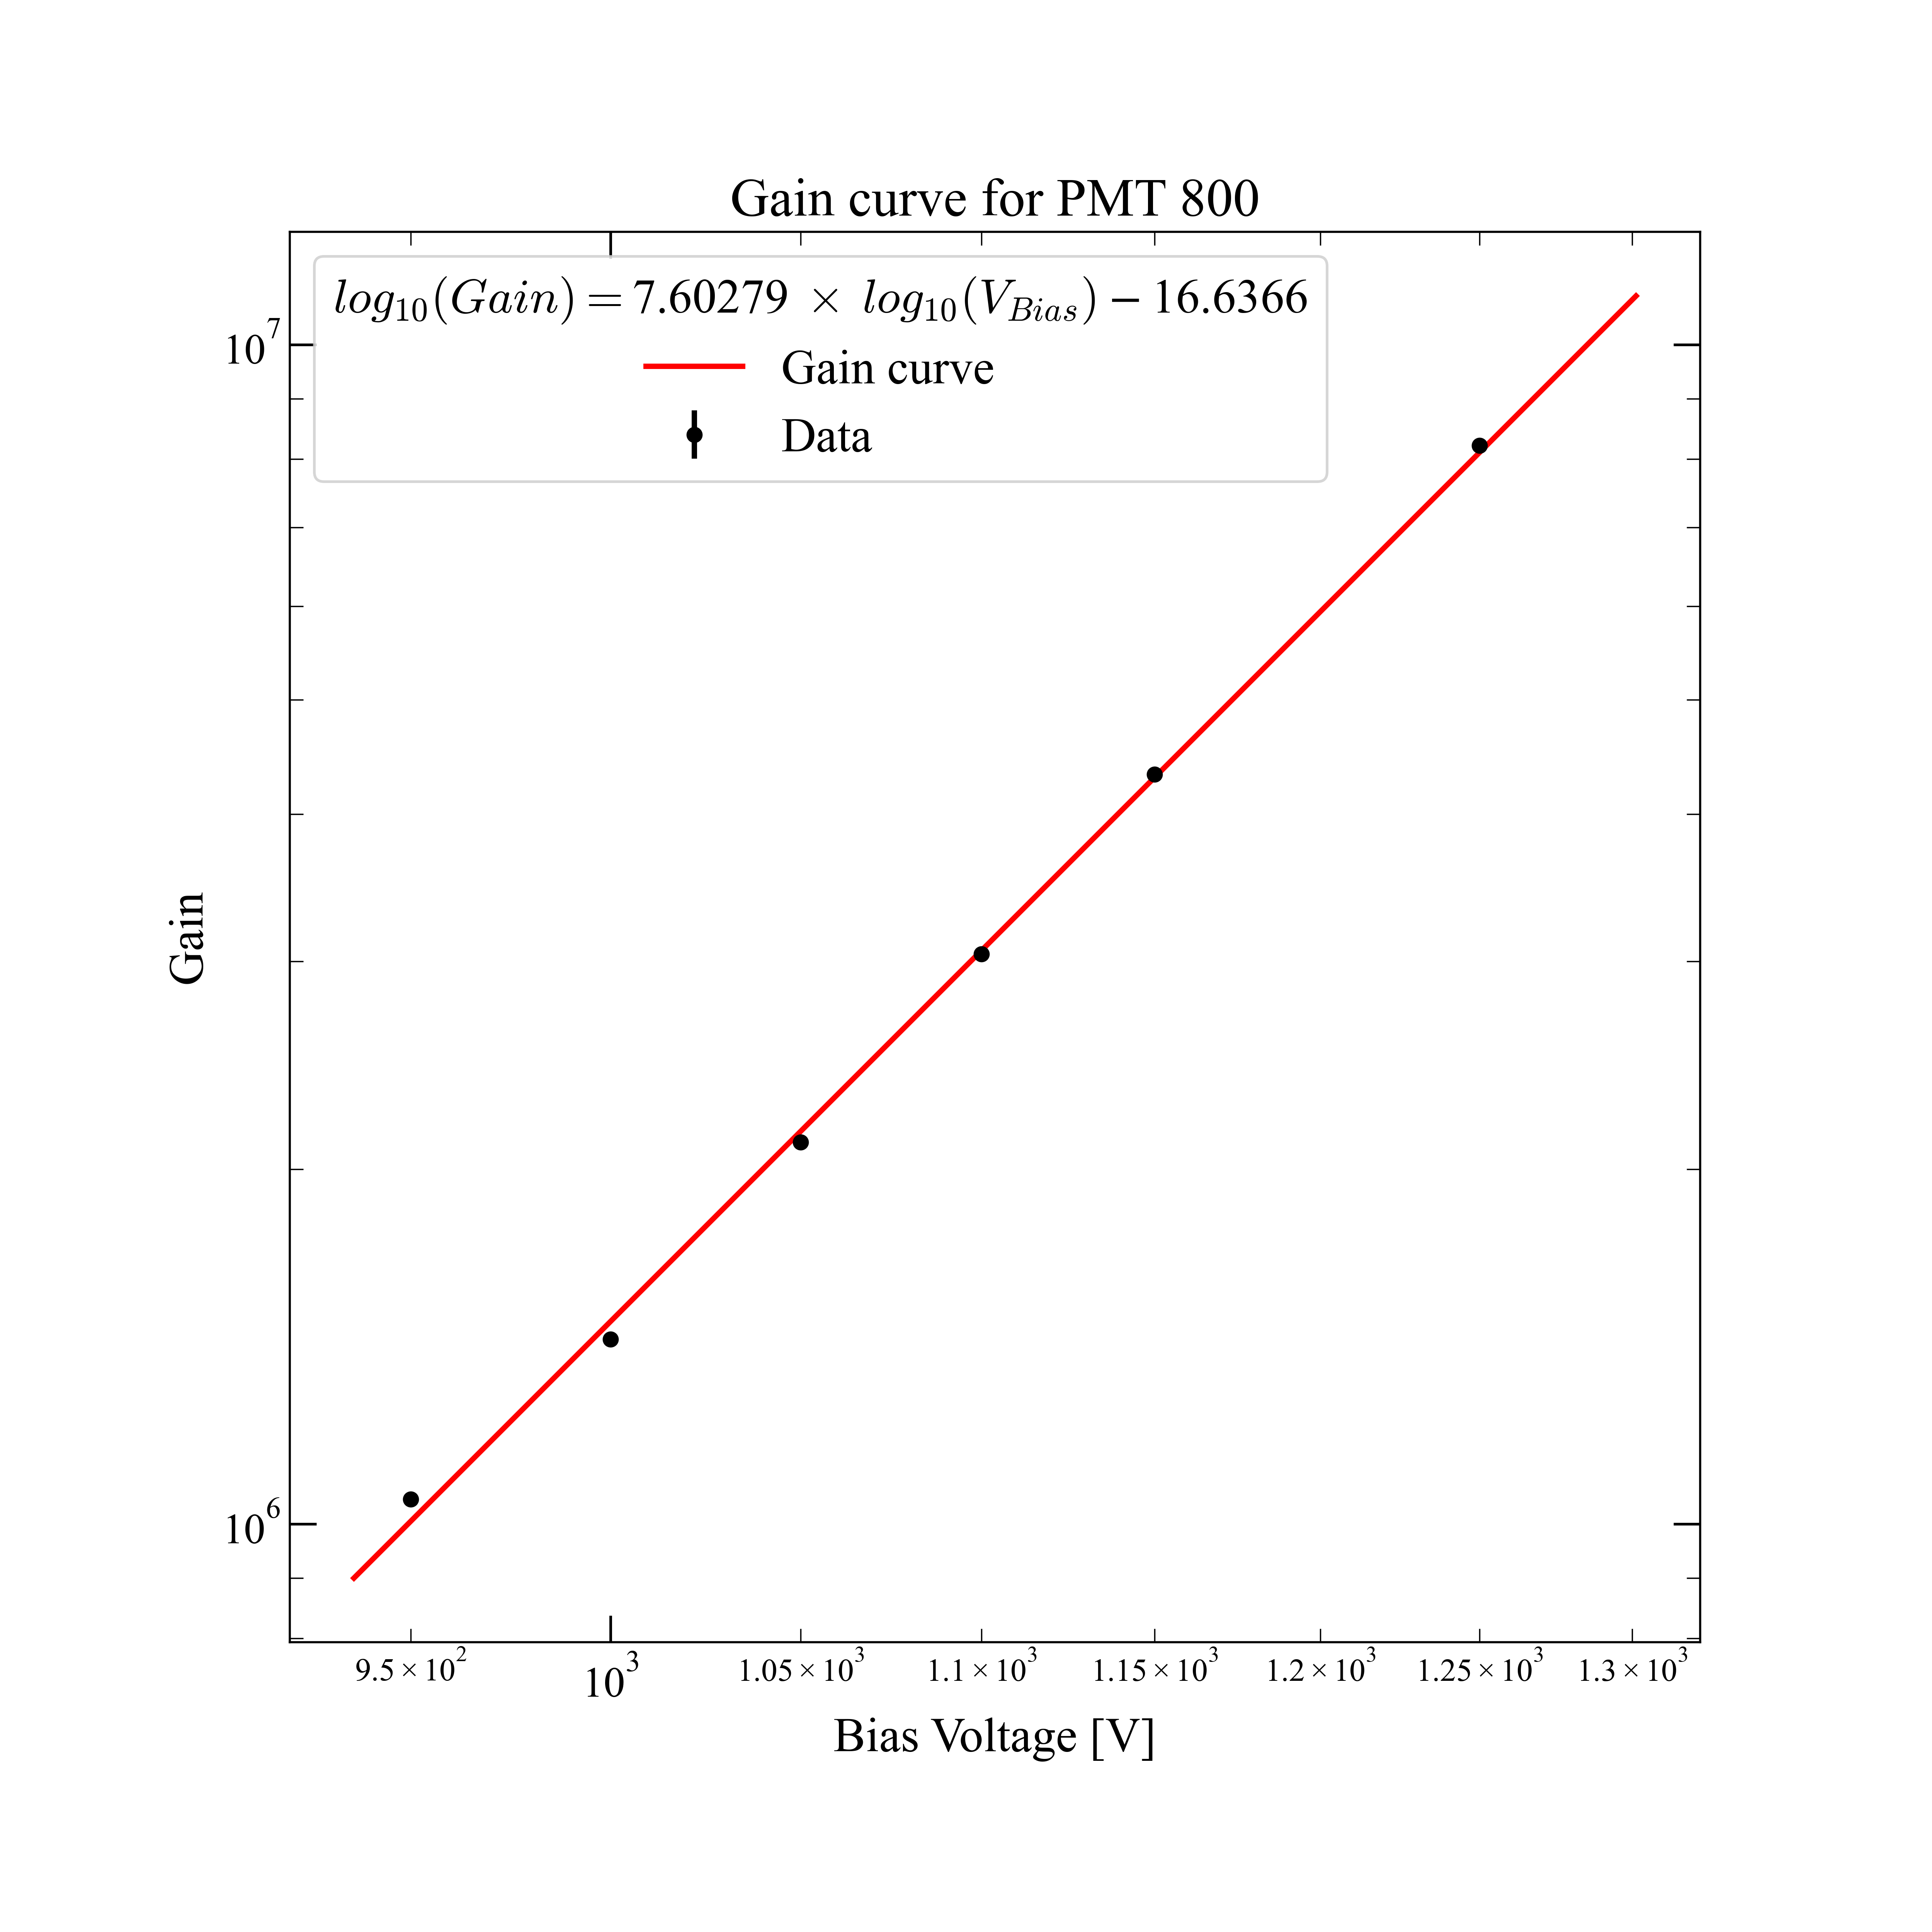
\includegraphics[width=\textwidth]{figures/ODCommissioning/PMT800_GainCurve.png}
     \end{subfigure}
     \hfill
     \begin{subfigure}[b]{0.47\textwidth}
         \centering
         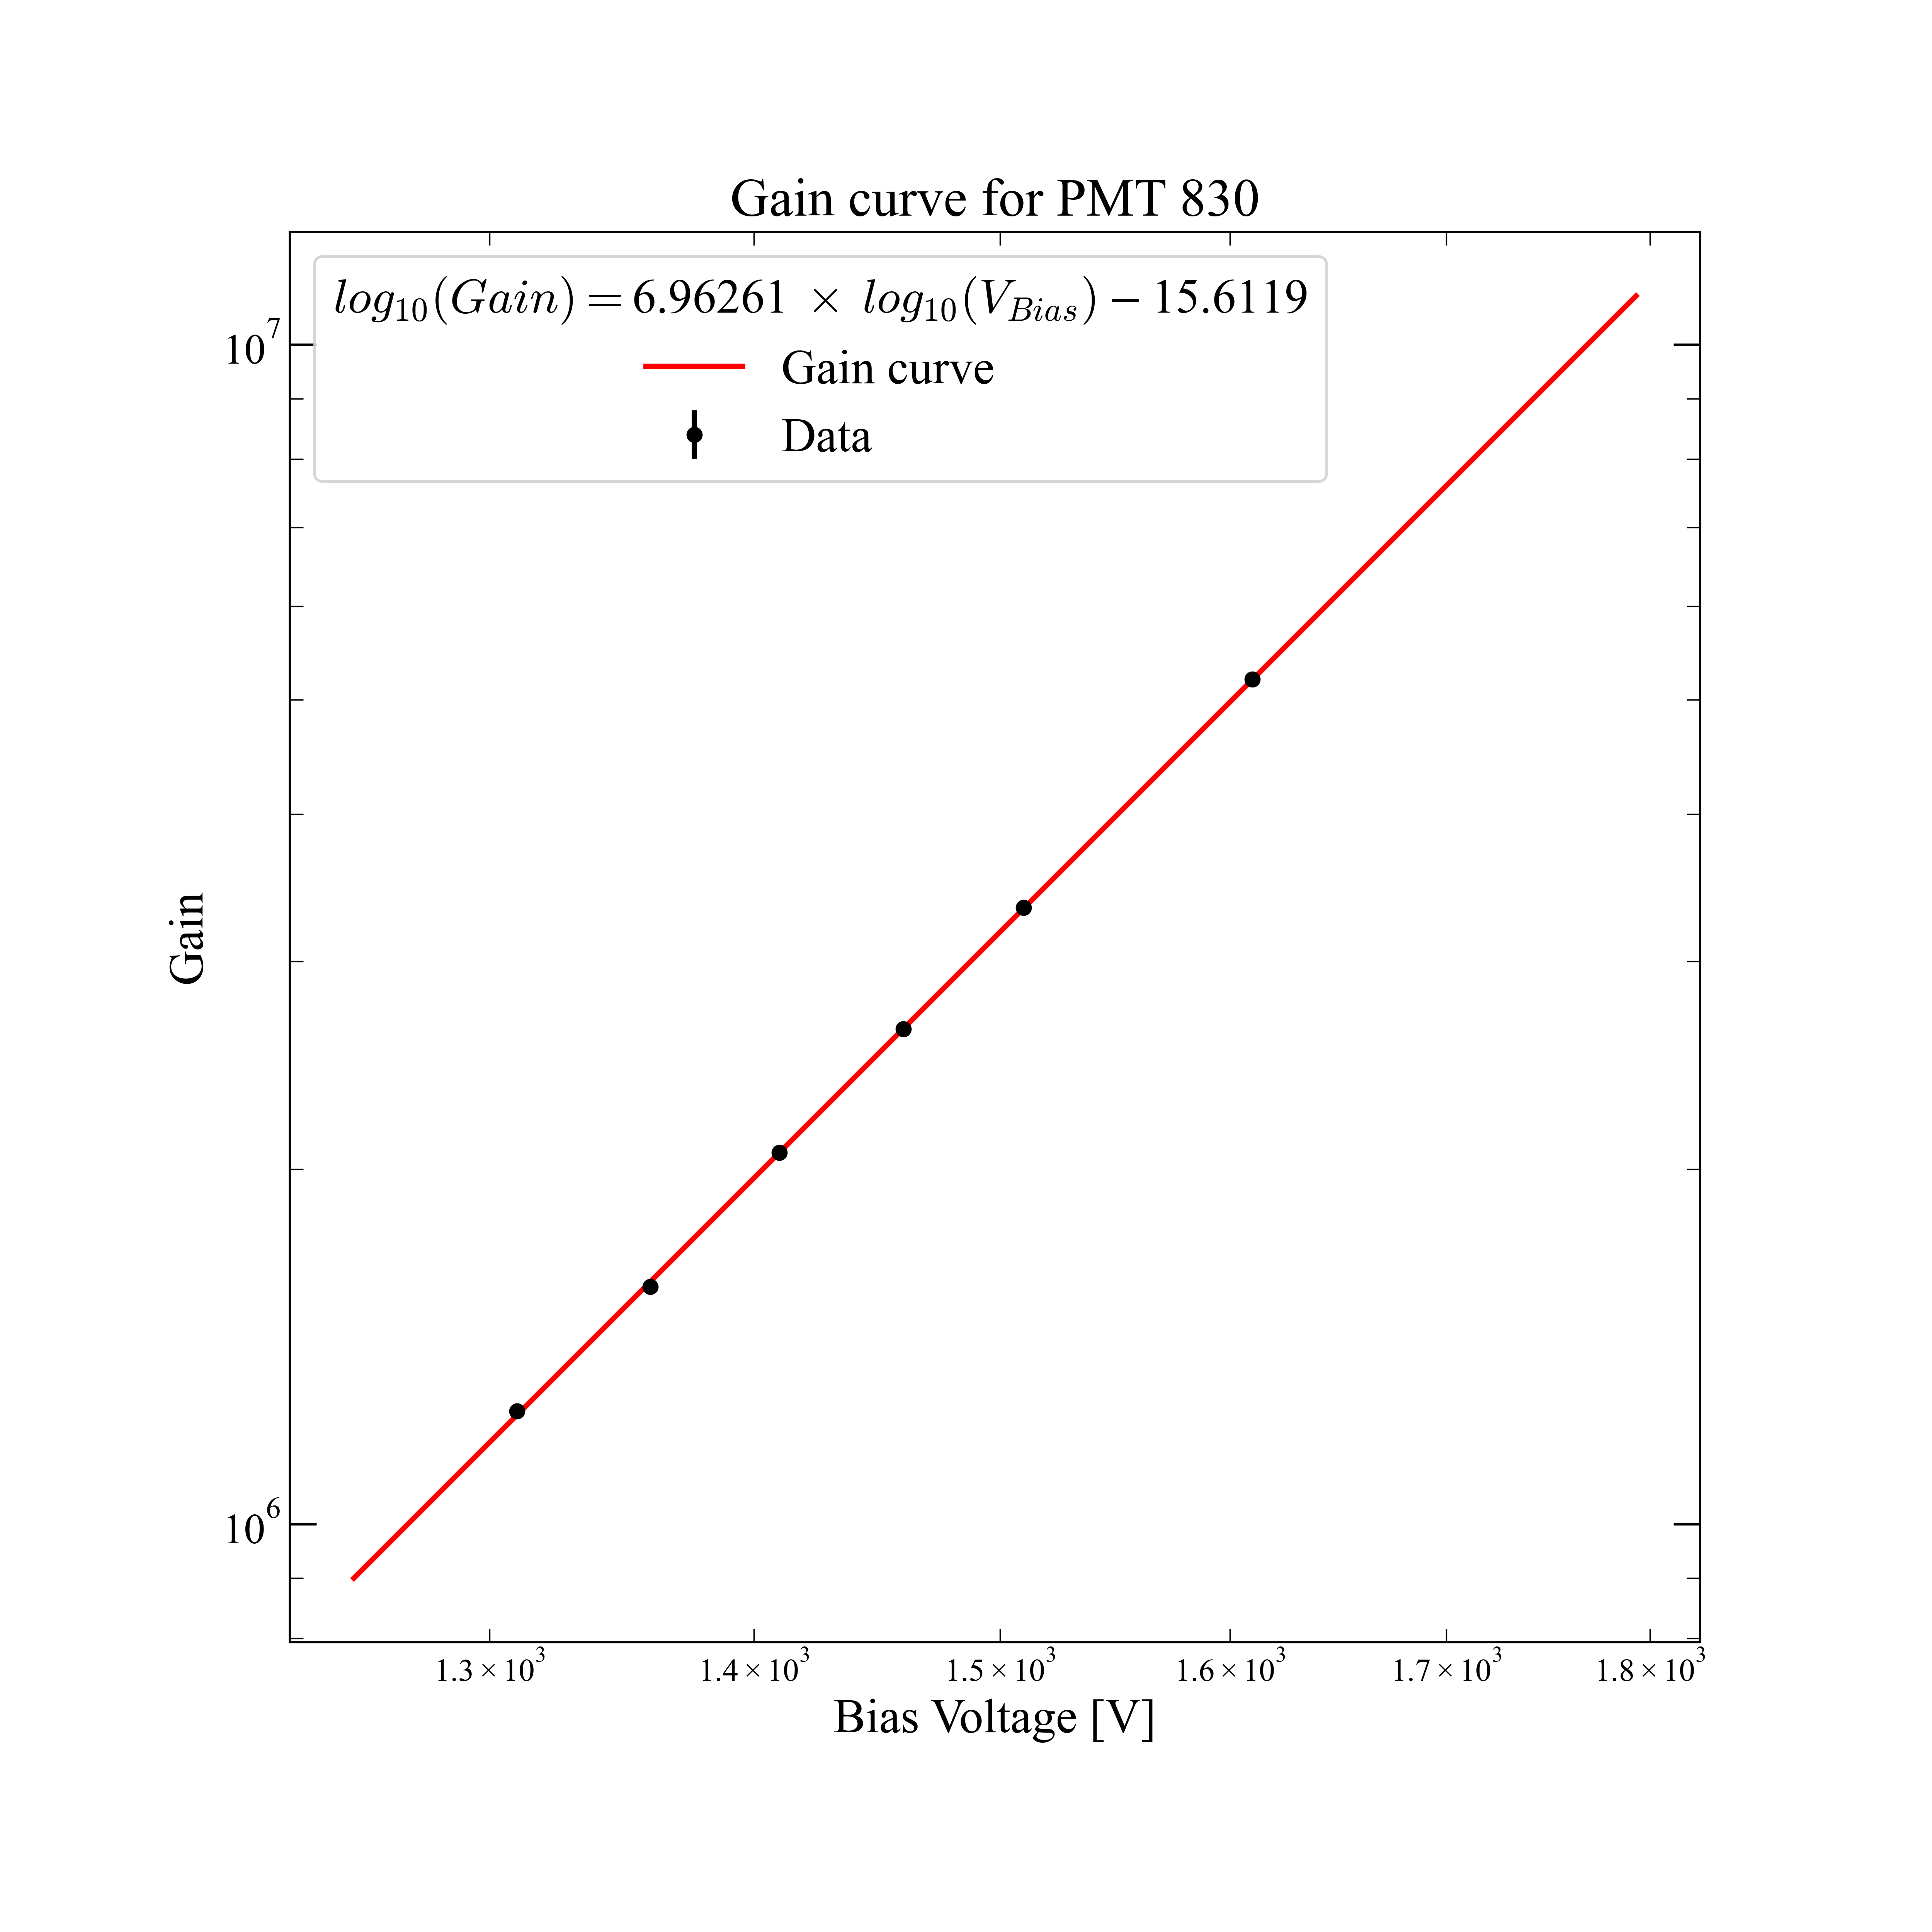
\includegraphics[width=\textwidth]{figures/ODCommissioning/PMT830_GainCurve.png}
     \end{subfigure}
     \hfill
     \begin{subfigure}[b]{0.47\textwidth}
         \centering
         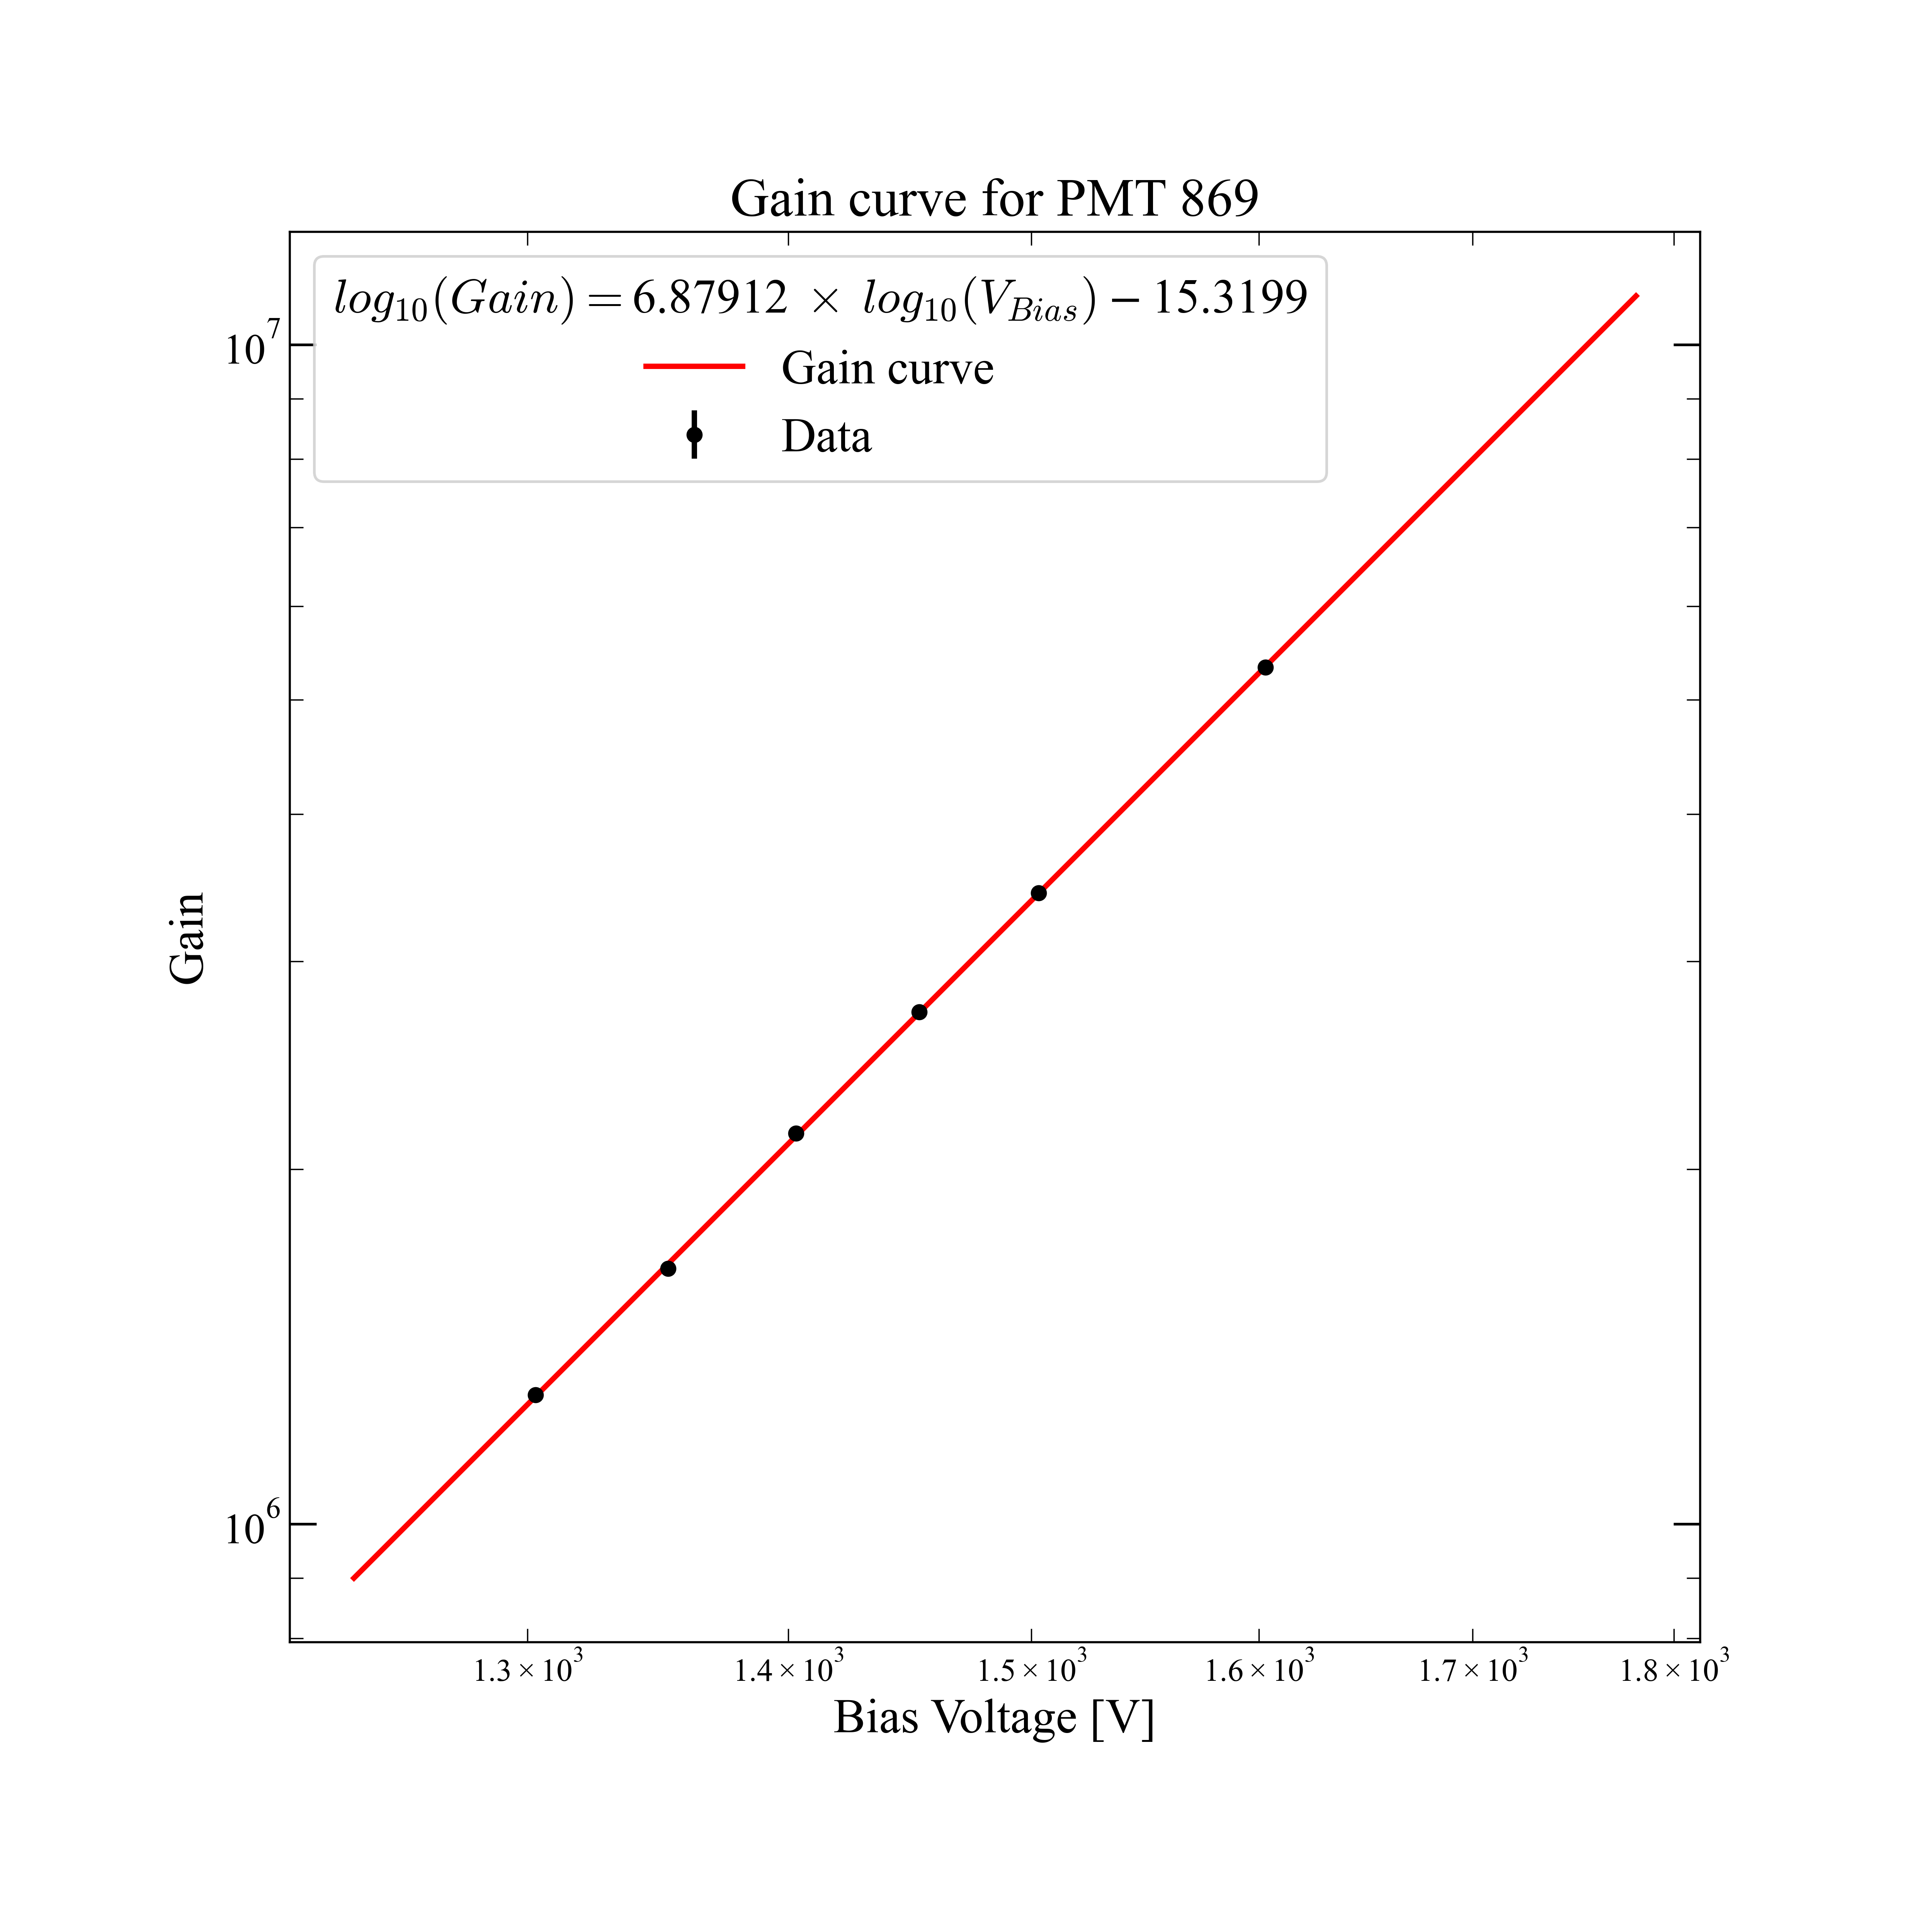
\includegraphics[width=\textwidth]{figures/ODCommissioning/PMT869_GainCurve.png}
     \end{subfigure}
     \hfill
     \begin{subfigure}[b]{0.47\textwidth}
         \centering
         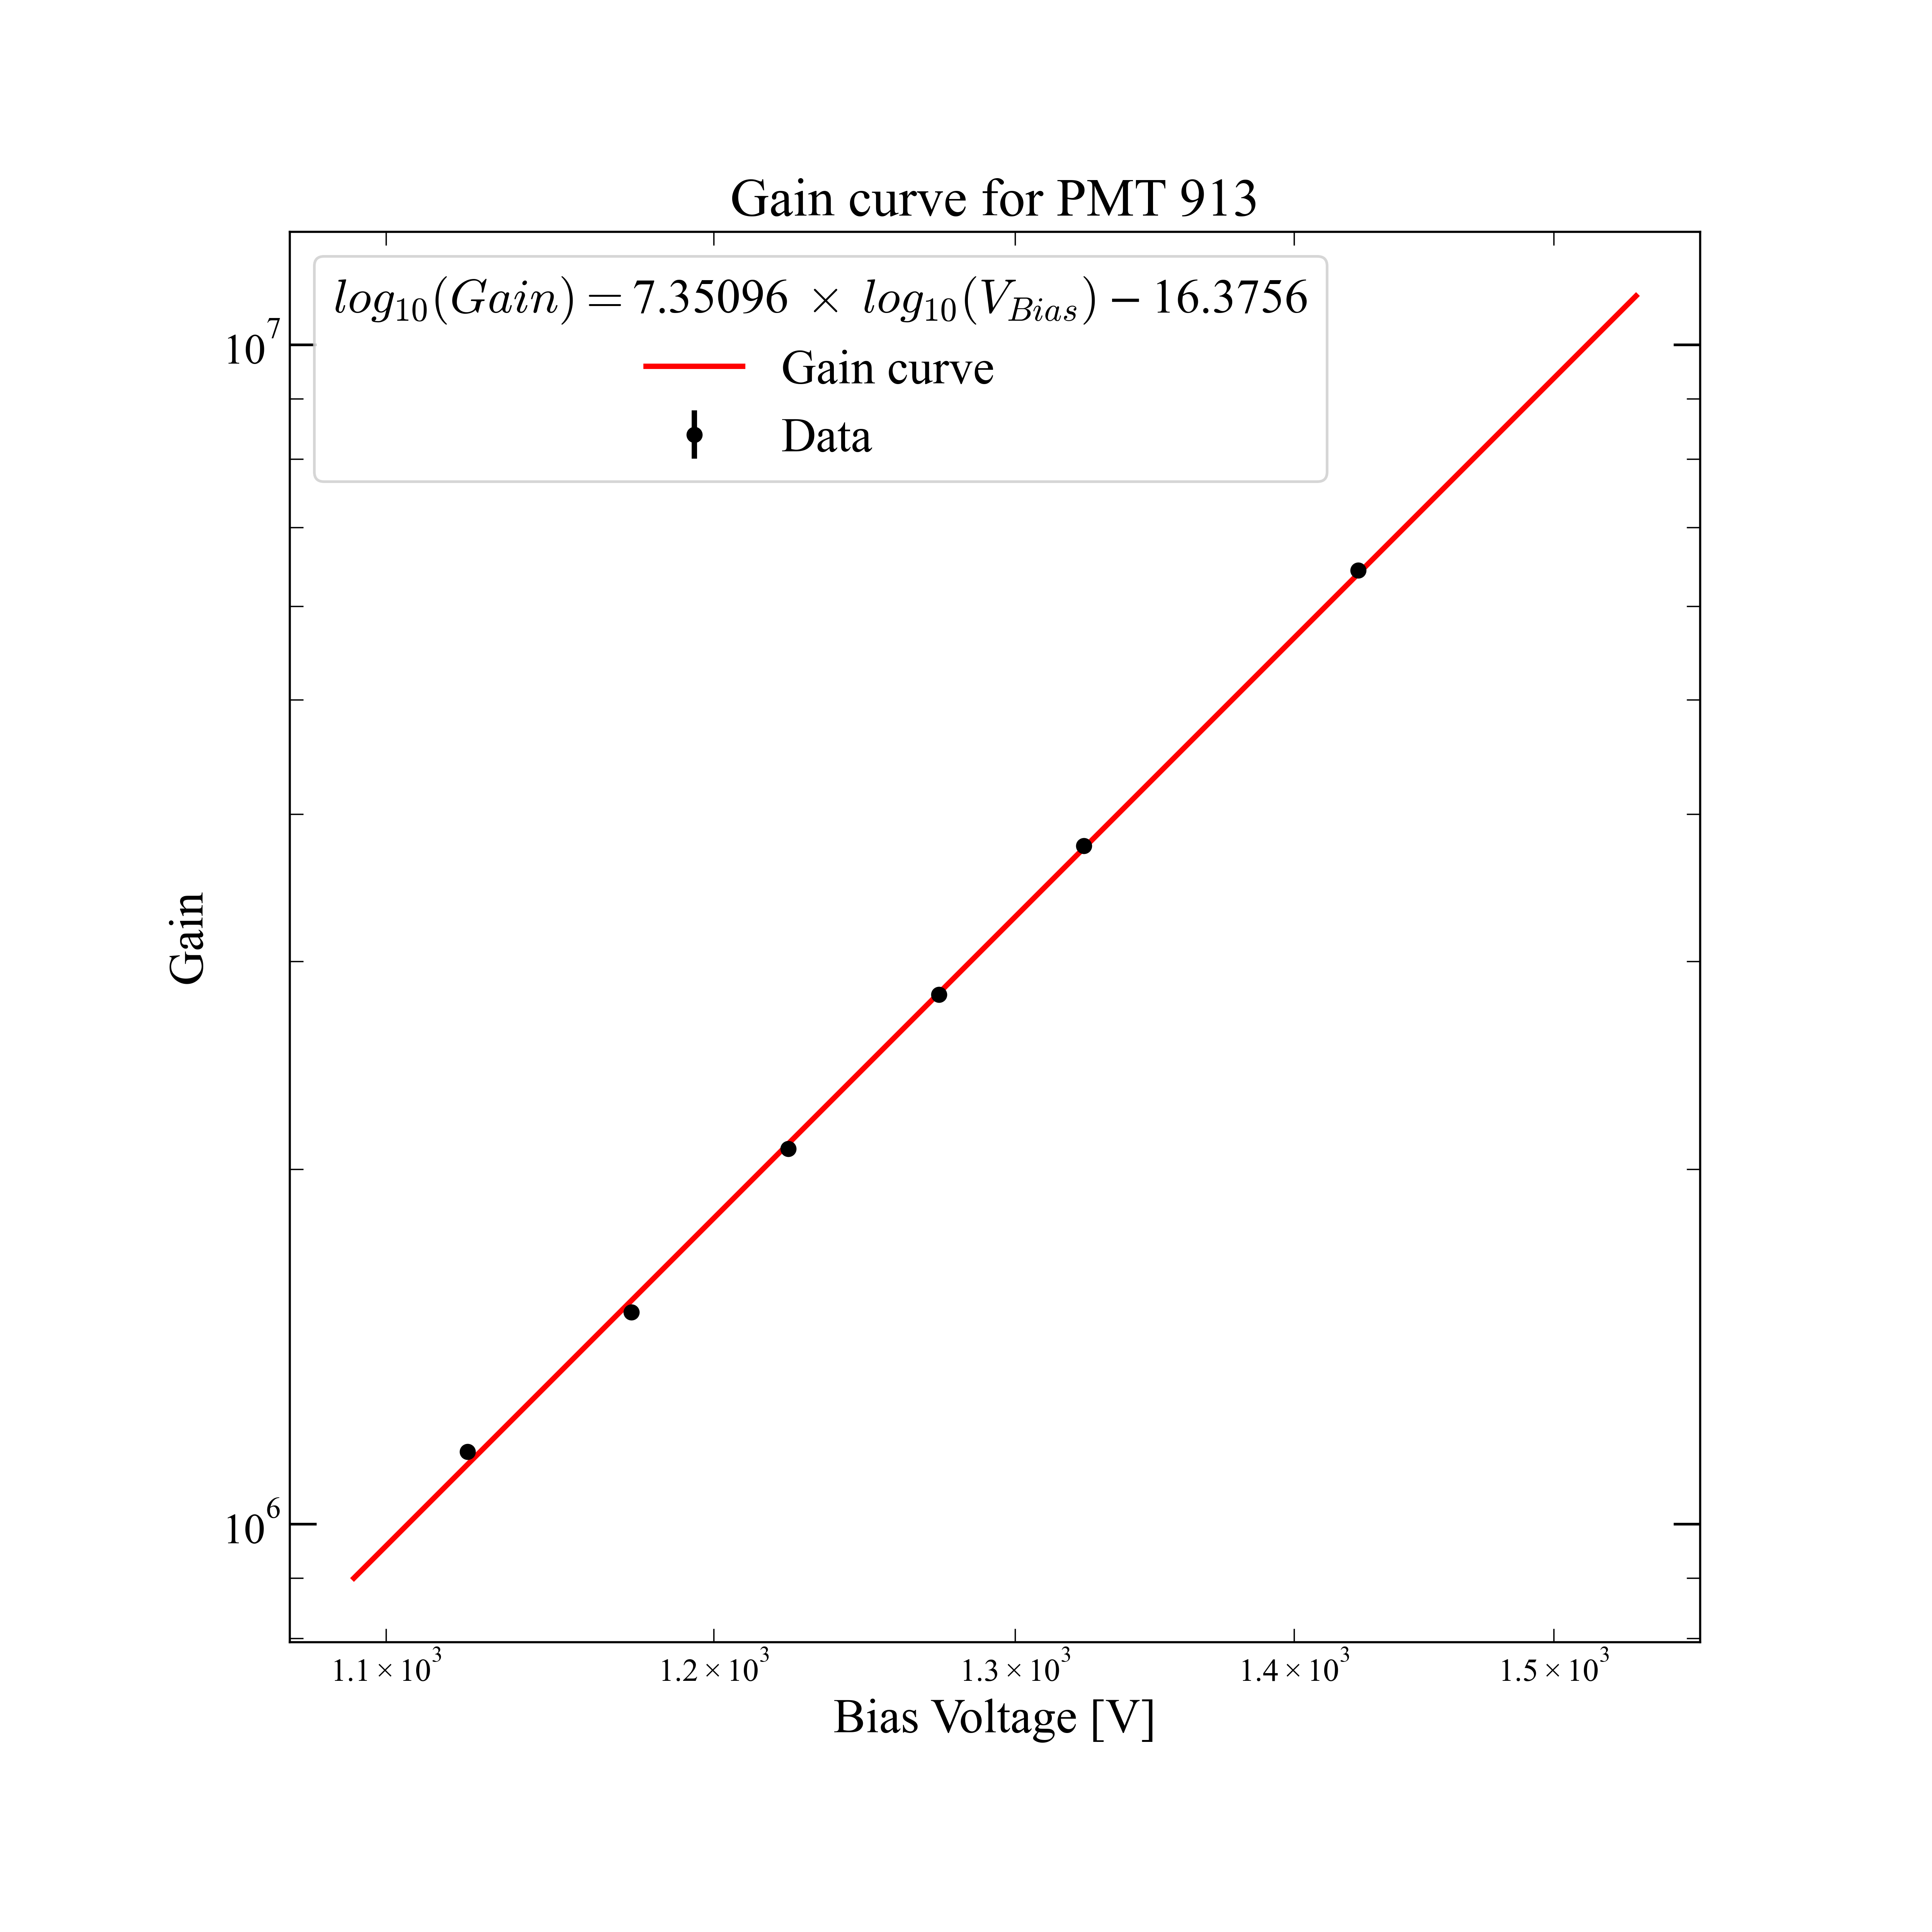
\includegraphics[width=\textwidth]{figures/ODCommissioning/PMT913_GainCurve.png}
     \end{subfigure}
        \caption{Four examples of gain curves for the OD PMTs measured prior to the start of the WS2024 campaign. The $\gamma$ factor varies between PMTs due to systematic differences in the surfaces of the dynodes and photocathode.}
        \label{fig:ODCommissioning/gainCurve}
\end{figure}

\begin{figure}[ht!]
    \centering
    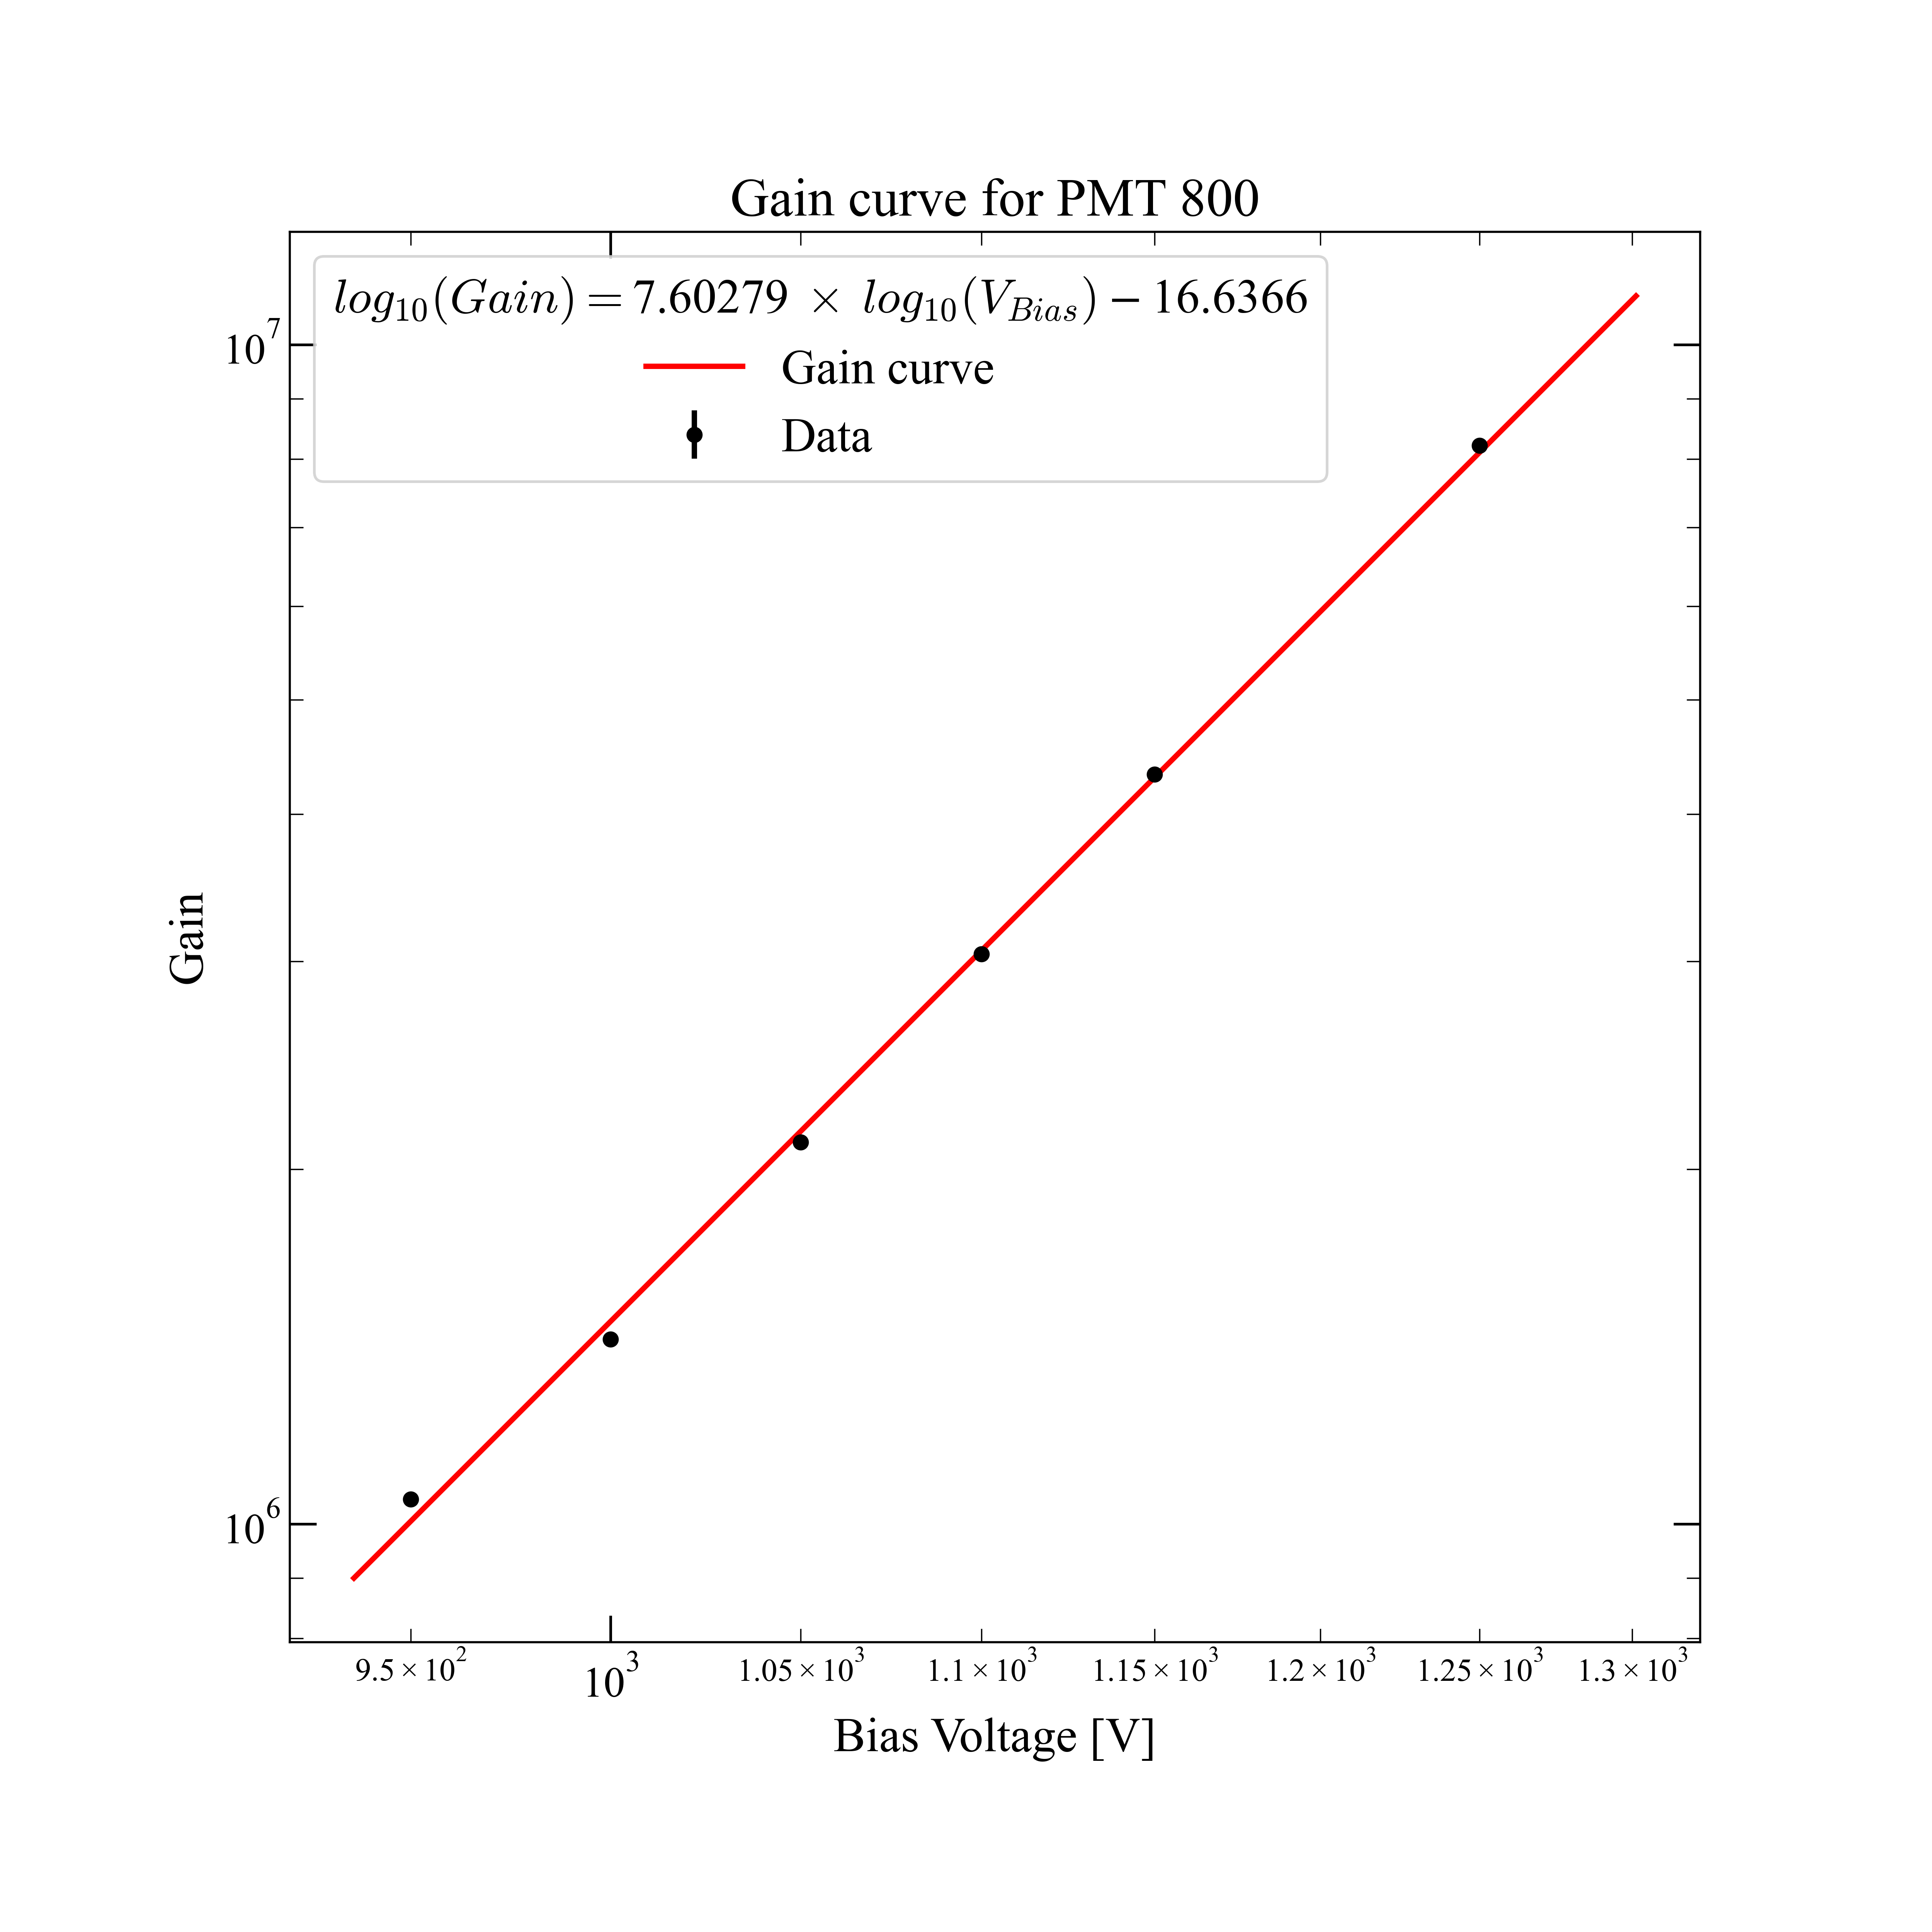
\includegraphics[width=0.7\linewidth]{figures/ODCommissioning/PMT800_GainCurve.png}
    \caption{Gain curve for PMT 800 measured measured prior to the start of the WS2024 campaign.}
    \label{fig:ODCommissioning/PMT800_gainCurve}
\end{figure}

\begin{figure}[ht!]
    \centering
    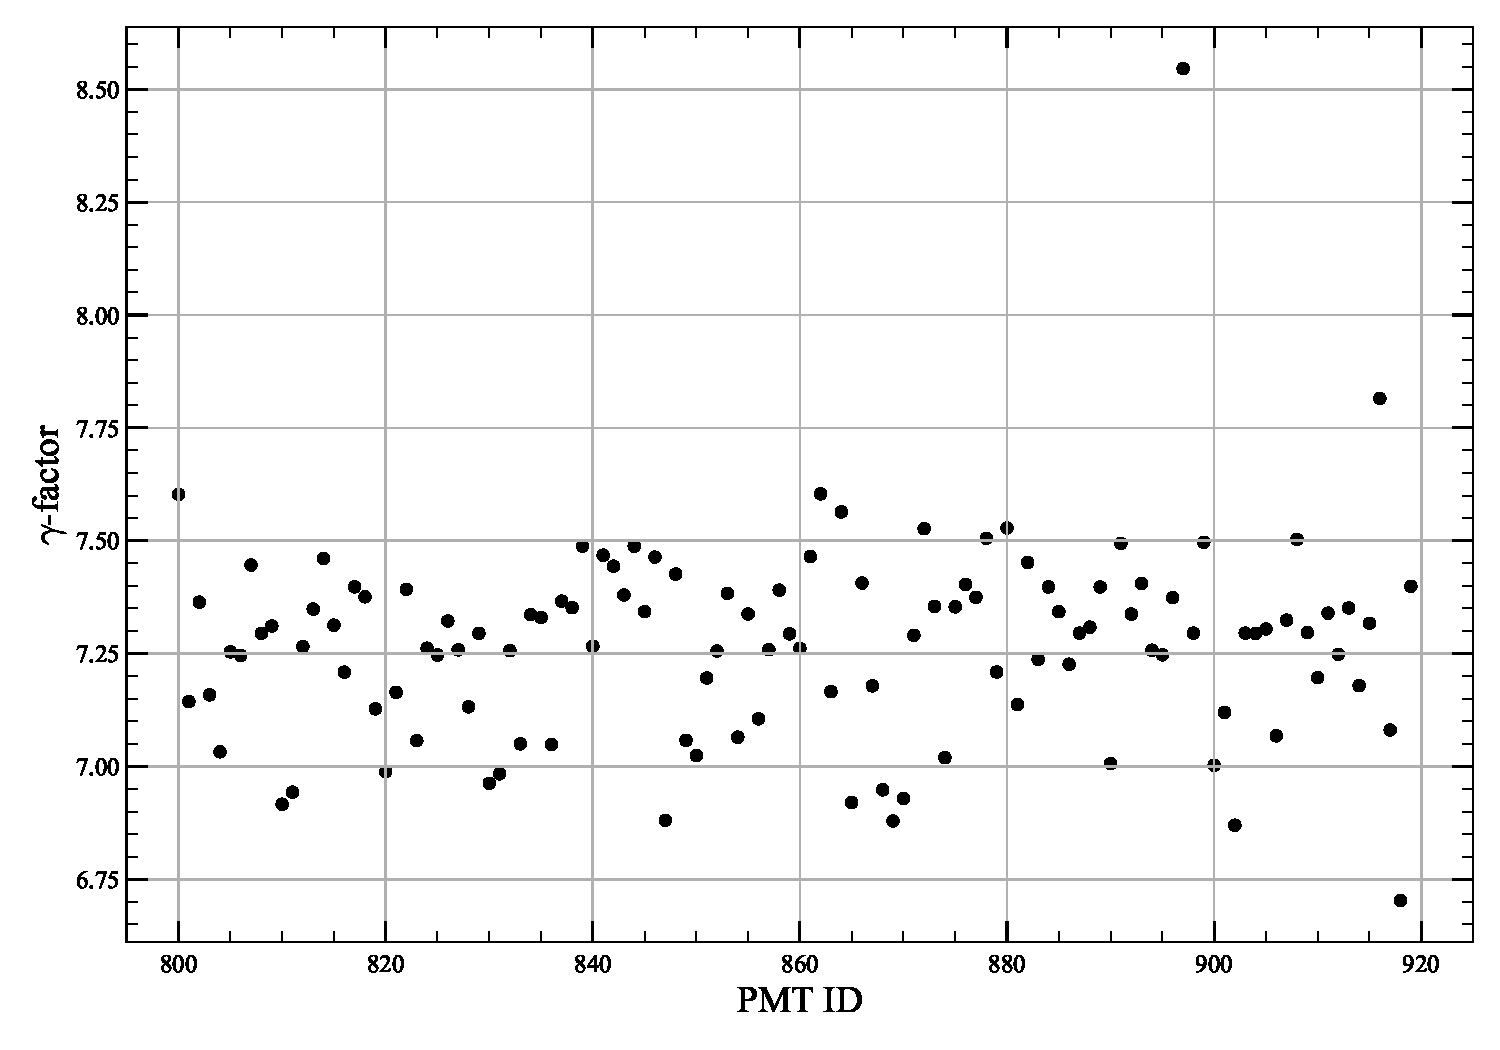
\includegraphics[width=0.7\linewidth]{figures/ODCommissioning/gammaFactorScatterPlot.pdf}
    \caption{$\gamma$-factors for each of the OD PMTs measured prior to the WS2024 campaign. The $\gamma$ factor varies between PMTs due to systematic differences in the surfaces of the dynodes and photocathode.}
    \label{fig:ODCommissioning/gammaFactors}
\end{figure}
\fi

\begin{figure}
     \begin{subfigure}[b]{0.4\textwidth}
         \centering
         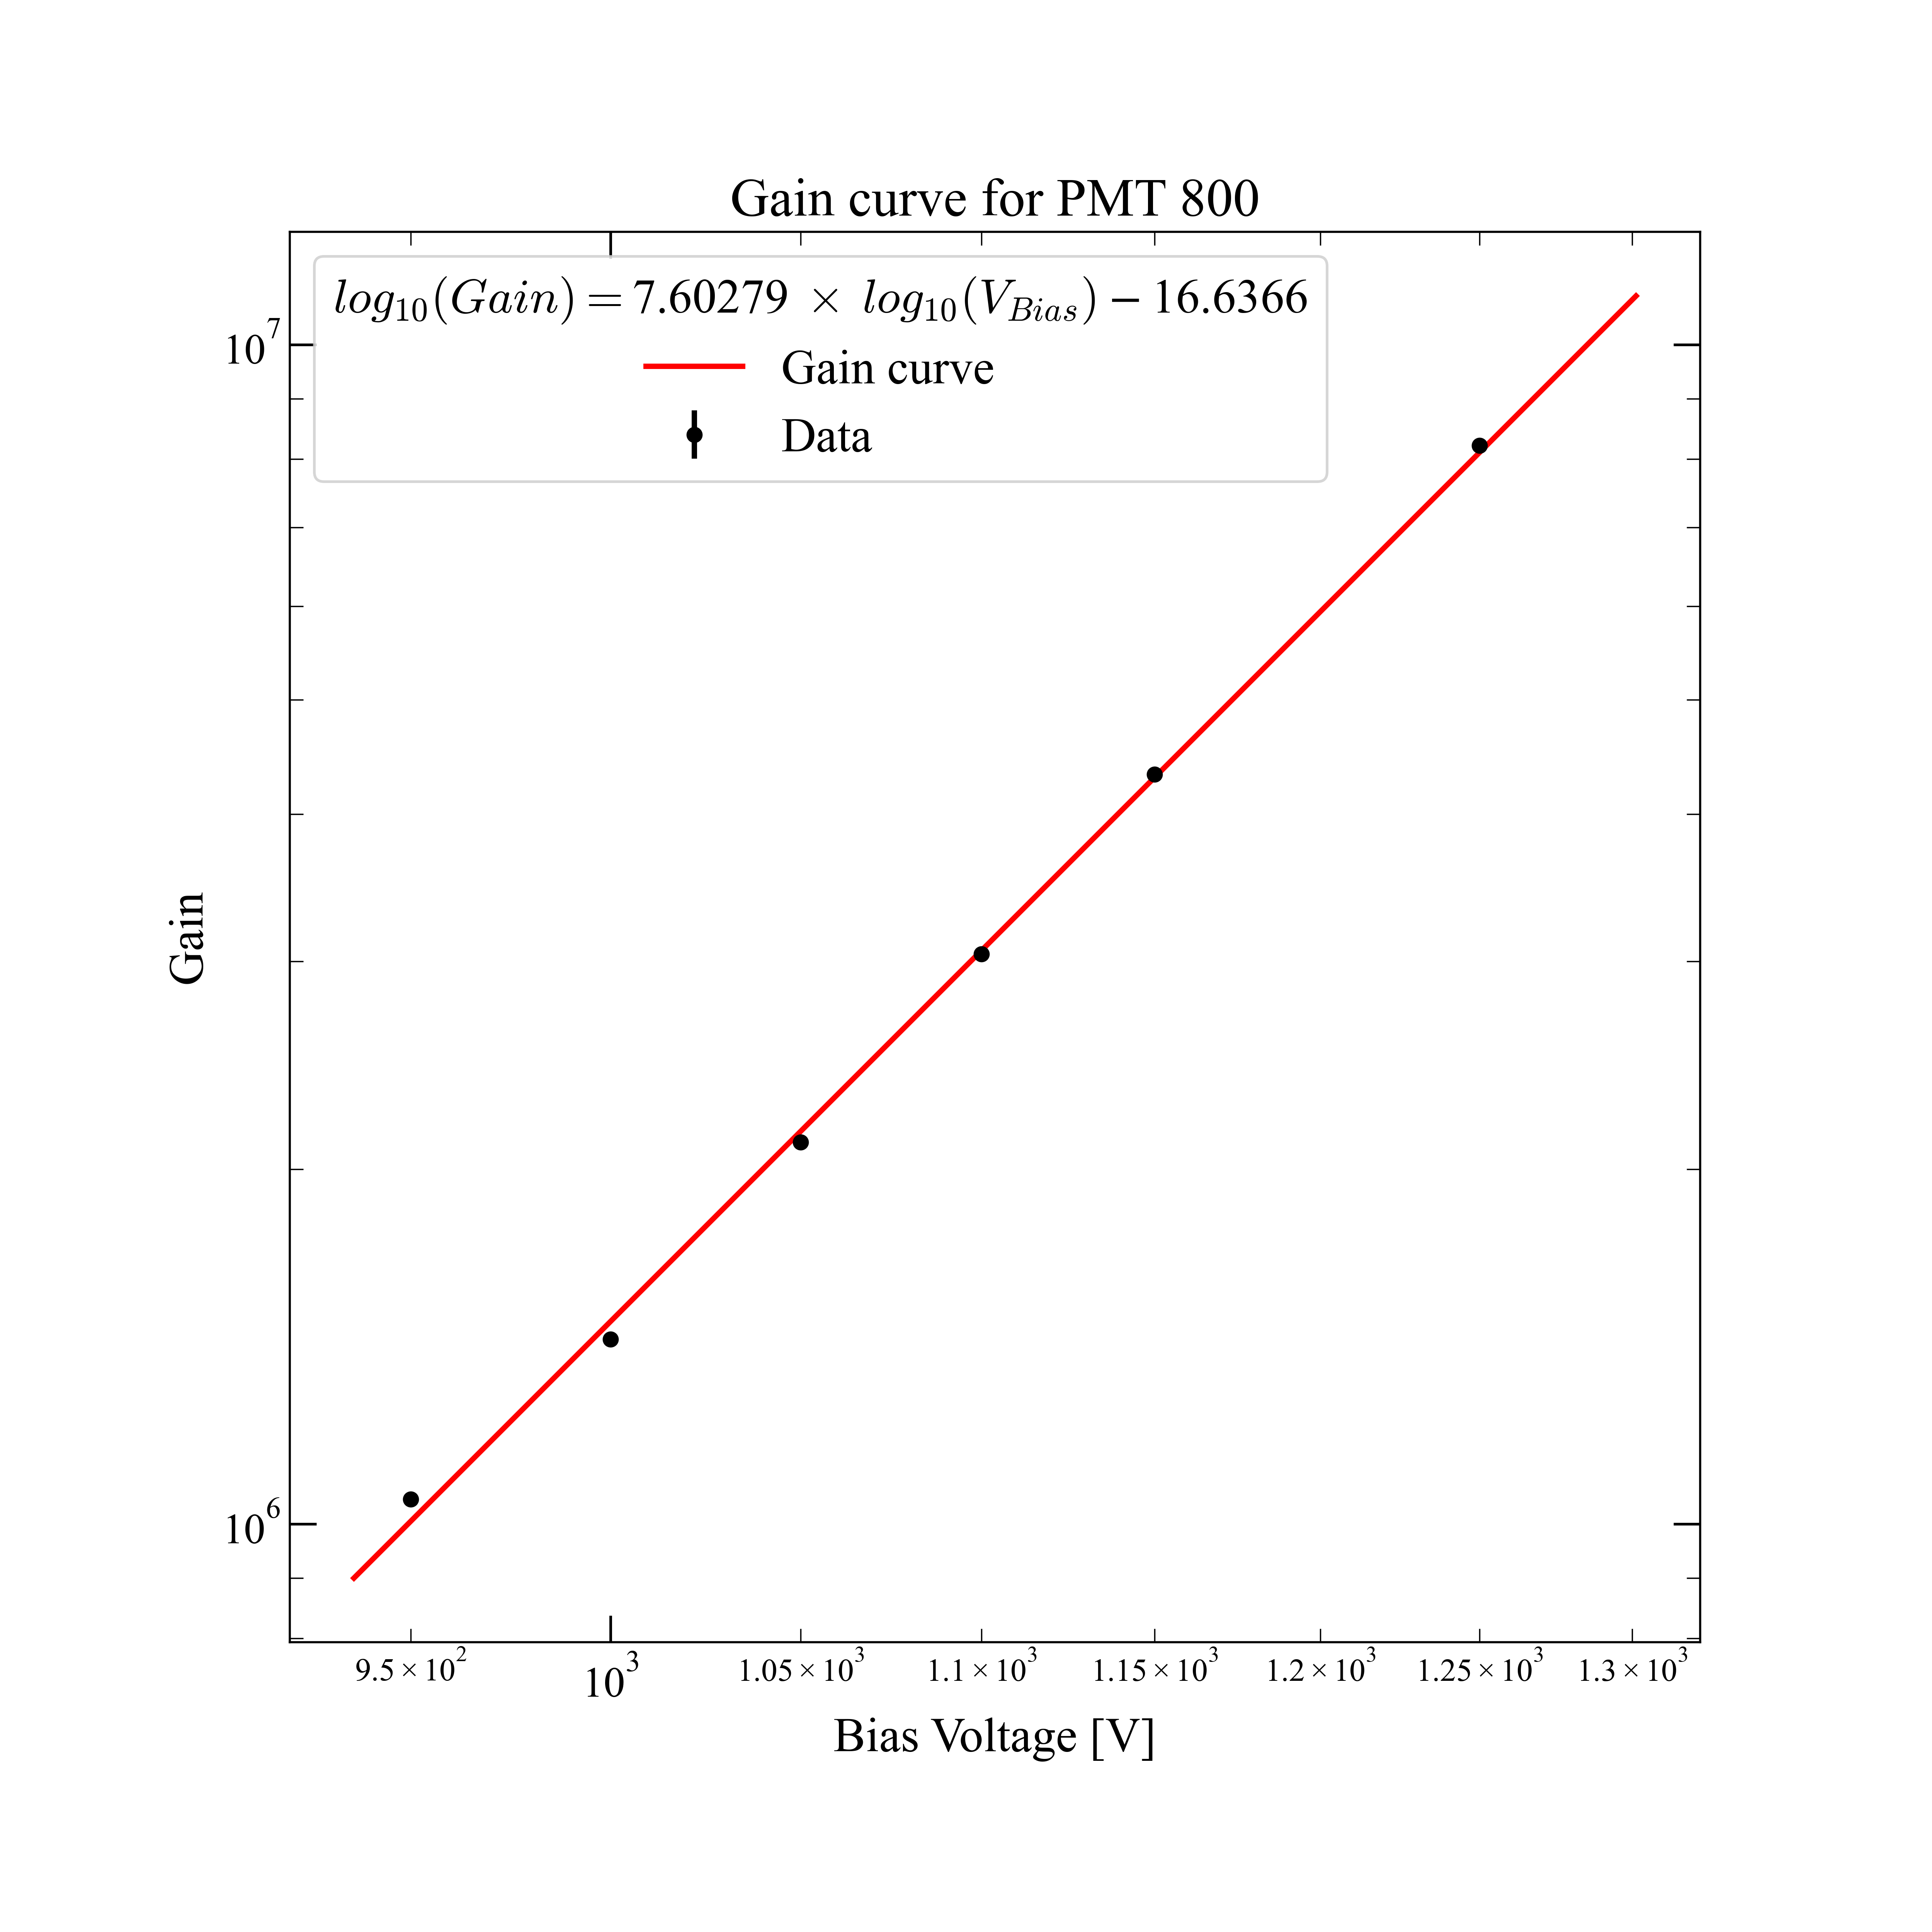
\includegraphics[width=\textwidth]{figures/ODCommissioning/PMT800_GainCurve.png}
         \caption{}
         \label{fig:ODCommissioning/PMT800_gainCurve}
     \end{subfigure}
     \hfill
     \begin{subfigure}[b]{0.59\textwidth}
         \centering
         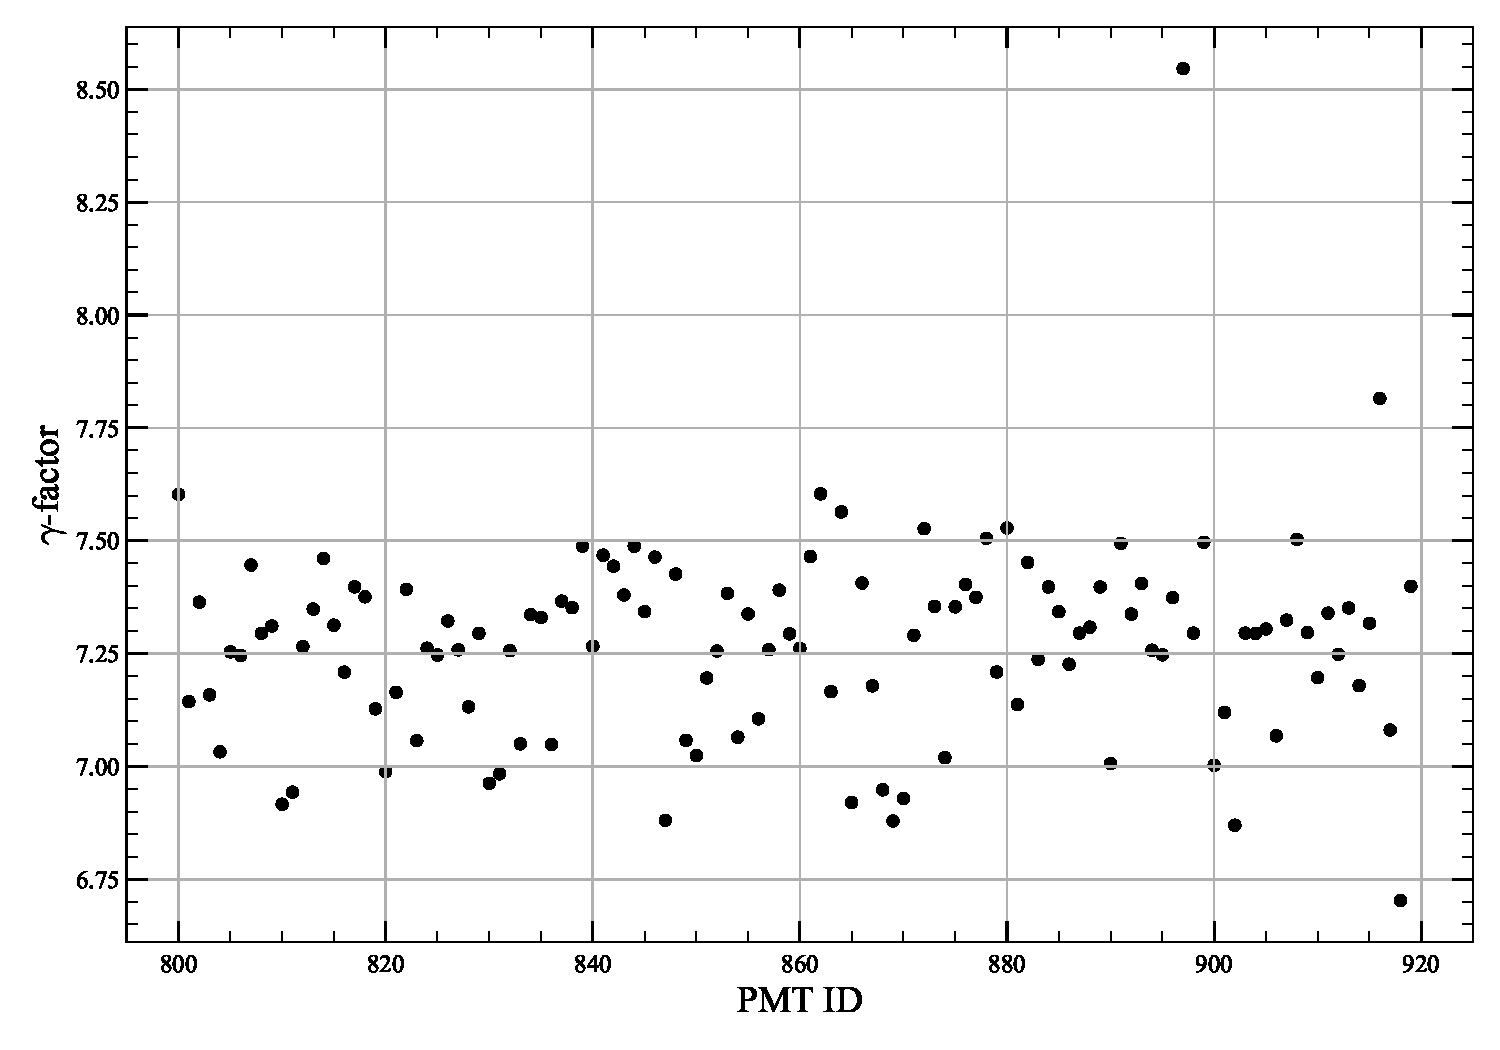
\includegraphics[width=\textwidth]{figures/ODCommissioning/gammaFactorScatterPlot.pdf}
         \caption{}
         \label{fig:ODCommissioning/gammaFactors}
     \end{subfigure}
        \caption{\textbf{Left:} Gain curve for PMT 800 measured measured prior to the start of the WS2024 campaign. \textbf{Right:} $\gamma$-factors for each of the OD PMTs measured prior to the WS2024 campaign. The $\gamma$ factor varies between PMTs due to systematic differences in the surfaces of the dynodes and photocathode.}
        \label{fig:ODCommissioning/gainCurve}
\end{figure}

\section{Optical calibration system development}\label{sec:ODCommissioning/OCSDevelopment}
\subsection{Monitoring PMT}\label{sec:ODCommissioning/MonitoringPMT}
One of the key components in the OD OCS is the monitoring PMT (mPMT), used for precise monitoring of the light intensity and system stability. The mPMT is a Hamamatsu R5912 PMT which is installed in a rack-mounted dark box close to the OCS electronics \cite{Turner:2021qvi}. This PMT is identical to those used in the OD. The stability of the light produced by the LEDs is monitored through the comparison of light produced by an in-situ YAP:Ce-Am pulser which produces light pulses corresponding to 5000 photoelectrons \cite{KOBAYASHI1994355}. The in-situ source is attached mechanically to the glass face of the PMT, as shown in \autoref{fig:ODCommissioning/MonPMT_YAPCeSource}.

\begin{figure}[ht!]
     \centering
     \begin{subfigure}[b]{0.47\textwidth}
         \centering
         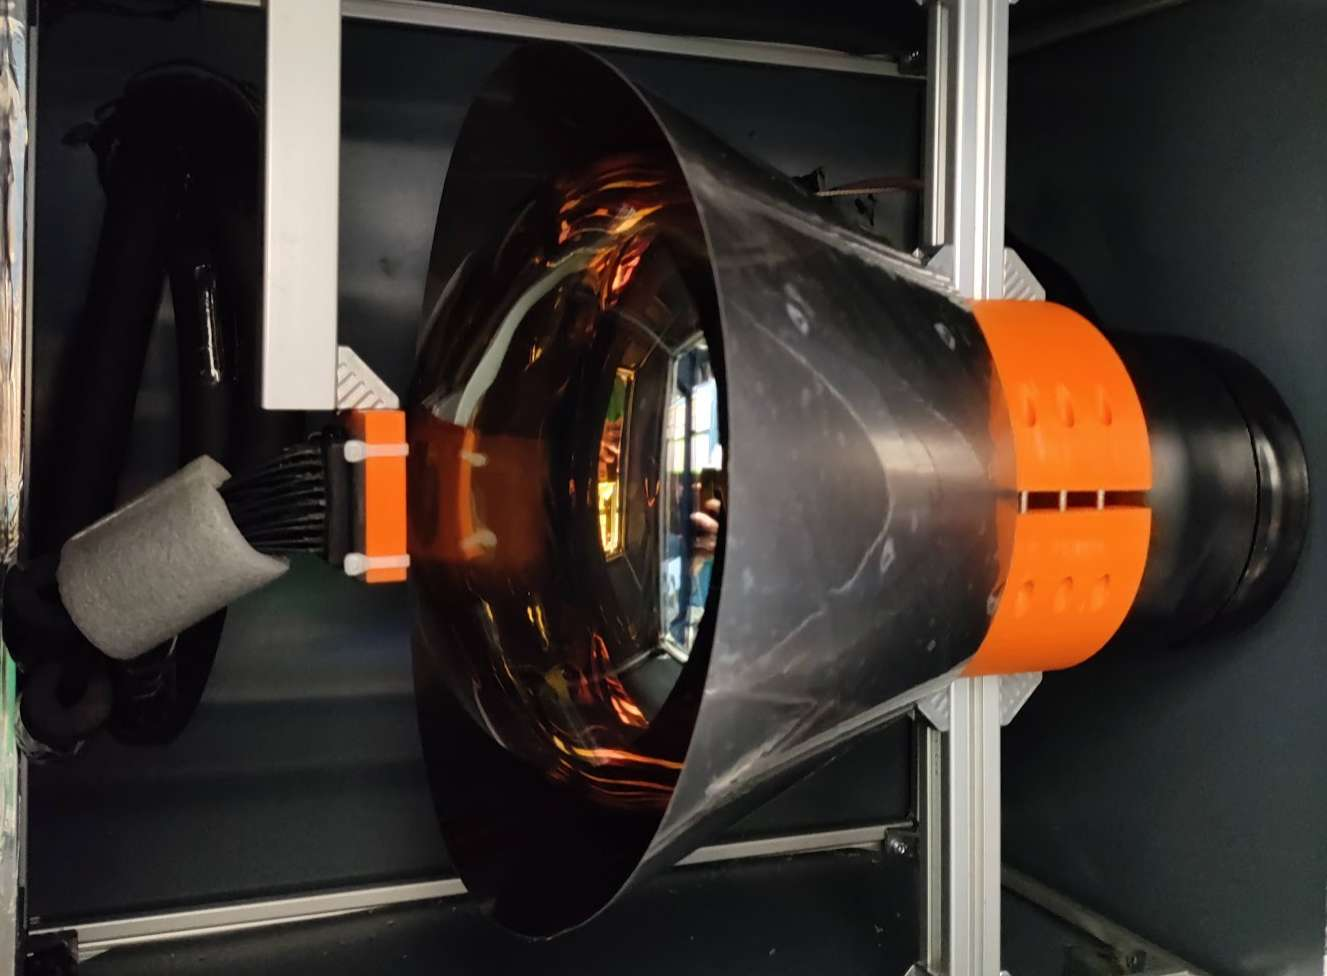
\includegraphics[width=\textwidth]{figures/ODCommissioning/MonitoringPMT.png}
     \end{subfigure}
     \hfill
     \begin{subfigure}[b]{0.47\textwidth}
         \centering
         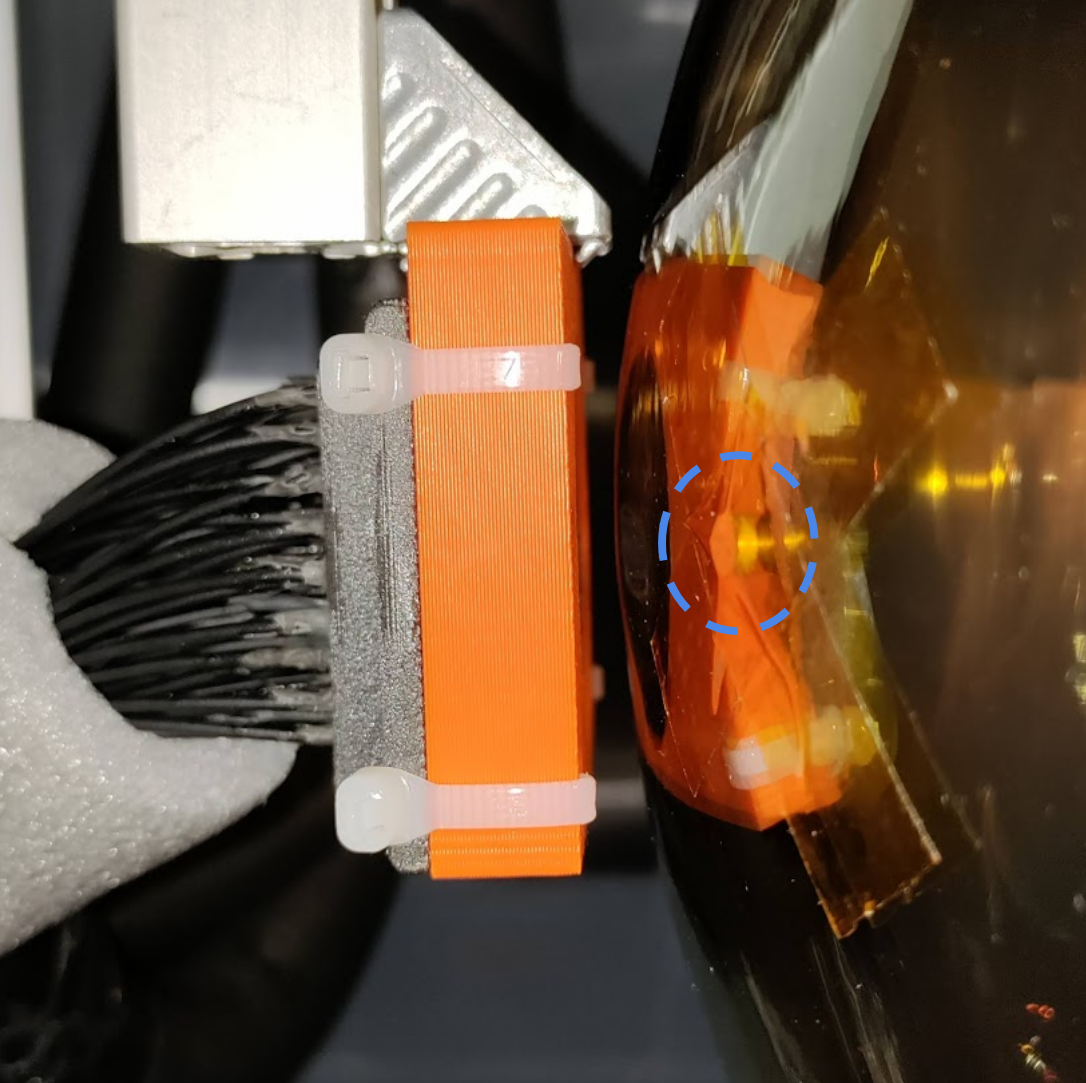
\includegraphics[width=0.74\textwidth]{figures/ODCommissioning/YAPCeSource.png}
     \end{subfigure}
        \caption{OD OCS Monitoring PMT. \textbf{Left:} The R5912 PMT mounted within the rack-mounted dark box situated beneath the OCS electronics. A coupler mounted in front of the PMT holds 40 single core fibres that carry light from the LEDs to the monitoring PMT. A mu-metal cone surrounding the PMT glass to reduce the impact of external electromagnetic forces on the photocathode and dynode chain. \textbf{Right: }Position of the YAP:Ce-Am source with respect to the PMT face. The source is mechanically attached to the glass using kapton tape.}
        \label{fig:ODCommissioning/MonPMT_YAPCeSource}
\end{figure}
Unlike the OD PMTs, the mPMT is biased to $1\times10^5$ gain at an operational voltage of 724~V. Due to the high intensity light produced by the YAP:Ce-Am source in such close proximity to the PMT, saturation effects were observed at a gain of $2\times10^6$ resulting in the desire to operate at the reduced gain to mitigate saturation.
\subsubsection{LZAP module development}
To process the RAW data from the PMT a custom LZAP module was developed called {\fontfamily{qcr}\selectfont ODOCSDarkboxPMTPulseFinder}. The module is similar in functionality to the module which is used to process data from the OD PMT array. From the RAW waveform data, the module is able to return the RQ-structured tree of the following variables, number of pulses in the event window, pulse ID of each pulse in the event window, pulse area of each pulse in the event window measured in mVns, start time of each pulse relative to when the event was triggered measured in ns, end time of each pulse relative to when the event was triggered measured in ns, the peak amplitude of each pulse measured in mV and the time at which the pulse reaches its peak amplitude relative to the trigger time measured in ns.
%\begin{itemize}
%    \item {\fontfamily{qcr}\selectfont int} Number of pulses in event window
%    \item {\fontfamily{qcr}\selectfont vector<int>} Pulse ID
%    \item {\fontfamily{qcr}\selectfont vector<float>} Pulse area [mVns] 
%    \item {\fontfamily{qcr}\selectfont vector<int>} Pulse start time relative to trigger [ns]
%    \item {\fontfamily{qcr}\selectfont vector<int>} Pulse end time relative to trigger [ns]
%    \item {\fontfamily{qcr}\selectfont vector<float>} Peak amplitude [mV]
%    \item {\fontfamily{qcr}\selectfont vector<int>} Peak time [ns]
%\end{itemize}
\subsubsection{Analysis}\label{sec:ODCommissioning/MonitoringPMTAnalysis}
Functionality tests of the {\fontfamily{qcr}\selectfont ODOCSDarkboxPMTPulseFinder} LZAP module were performed using an ALPACA analysis module to understand the peaks observed in the pulse area spectrum of the mPMT. It was assumed that the intensity of the light produced by the source would remain constant between OCS measurements. Using data collected for SPhE and afterpulsing\footnote{Afterpulses are spurious pulses that appear in the wake of the true signal pulse and have two main causes: light emitted by electrodes due to electron bombardment, and ionization of residual gas traces within the PMT. Further details on afterpulsing can be found in Ref.\cite{lkorley:thesis}} measurements, the peak produced by the YAP:Ce-Am source was identified. An example of this is shown in \autoref{fig:ODCommissioning/mPMTPADist}. The peak can be easily identified by overlaying the pulse spectra of the SPhE and afterpulsing measurements. This due to the different light intensity used for the measurements with peaks centred at 19300~mVns and 136000~mVns. The peak produced by the source is located at 42000~mVns.
\begin{figure}[ht!]
    \centering
    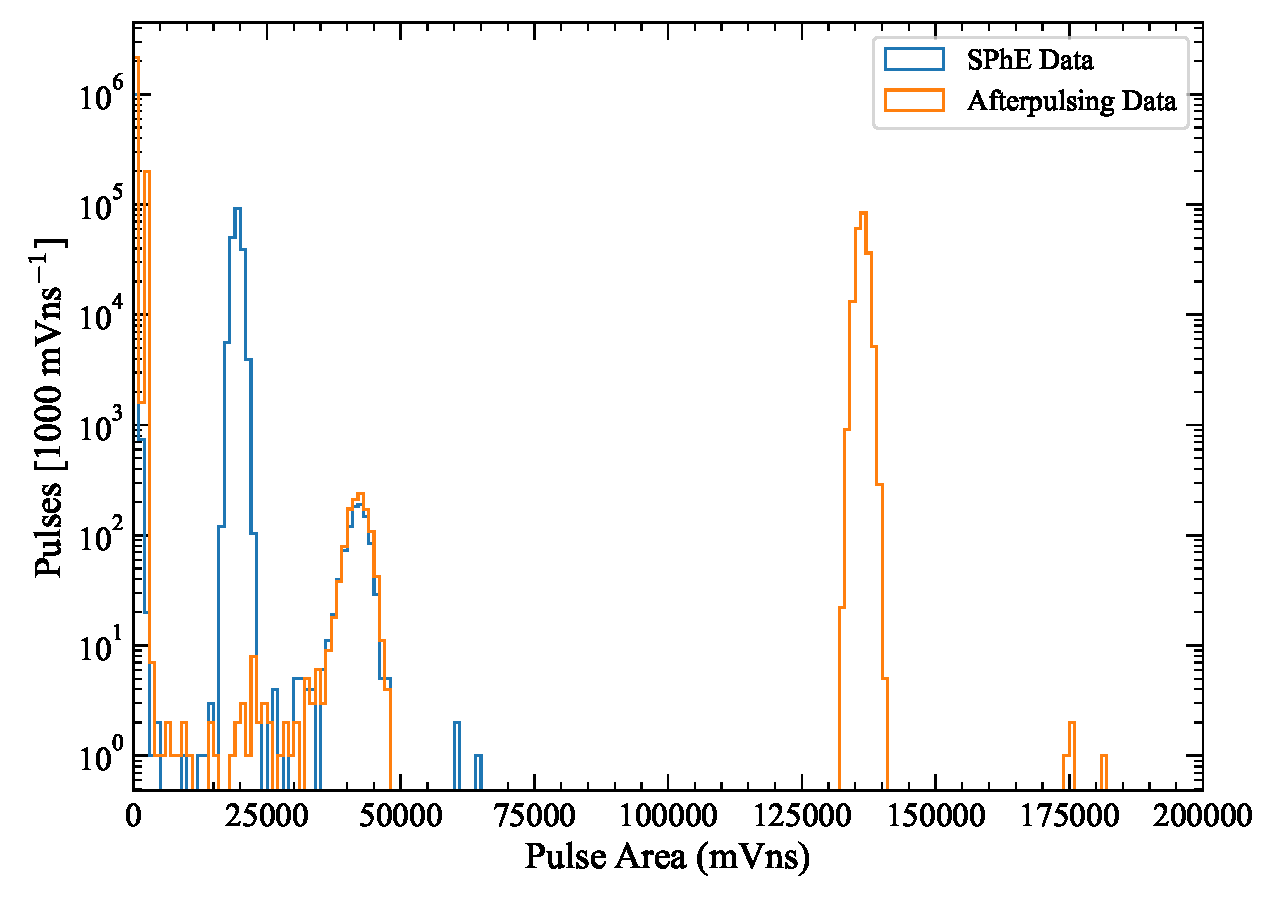
\includegraphics[width=0.7\linewidth]{figures/ODCommissioning/mPMT_PulseAreaSpectrum.pdf}
    \caption{Pulse area spectra from two OCS measurements. During the development of the OCS mPMT, this plot was used to determine the peak position of the light produced by the YAP:Ce-Am pulser. The peak can be easily identified by overlaying the pulse spectra of the SPhE and afterpulsing measurements. This due to the different light intensity used for the measurements with peaks centred at 19300~mVns and 136000~mVns. The peak produced by the source is located at 42000~mVns.}
    \label{fig:ODCommissioning/mPMTPADist}
\end{figure}
To select the OCS pulse independent of pulse area, a similar method of selection was used to that discussed in \autoref{sec:ODComissioning/SPhECalib}. However, due to the shorter fibres connecting the LEDs to the mPMT dark box the selection of pulses between 400~ns to 500~ns after the DAQ was triggered by the OCS. The pulses produced by the source occur randomly due to the radioactive decay of the $^{241}\text{Am}$, so pulse area criteria was used to select the pulses produced by the source based on a $\pm2\sigma$ selection away from a mean pulse area of 42000~mVns.

\pagebreak

\section{Concluding remarks}
The OD of LZ plays a crucial role in suppressing backgrounds for the direct detection of WIMPs. The primary purpose of the OD is to detect neutron interactions which have coincidence signals within the TPC. Neutrons which scatter in the TPC and then go on to capture on gadolinium or hydrogen or recoil off protons produce energy deposits of $\sim100$~keV. The pulses of light detected by PMTs in the OD for such low energy interactions are $\sim15$~photons in size and require PMTs to be calibrated to a single photon sensitivity. A model of photomultiplier response to single photoelectrons is presented alongside the single photoelectron calibration of the Hamamatsu R5912 PMT. A dedicated optical calibration system is used calibrated the OD PMT single photon electron response. An \textit{in situ} monitoring system is used to monitor the light output of the LEDs which are used for the single photon electron calibration measurements. The reconstructed gain of the OD PMTs is measured and average gain change of $(1.37\pm0.25)\%$ during the WS2024 science run is observed. Understanding the response of the OD PMTs and the stability of the single photoelectron signal during science runs is imperative to the performance of the veto detectors and their ability to effectively identify events which coincident signals in the TPC.